\chapter{绪论}

{\textbf 【知识体系】}
\begin{center}
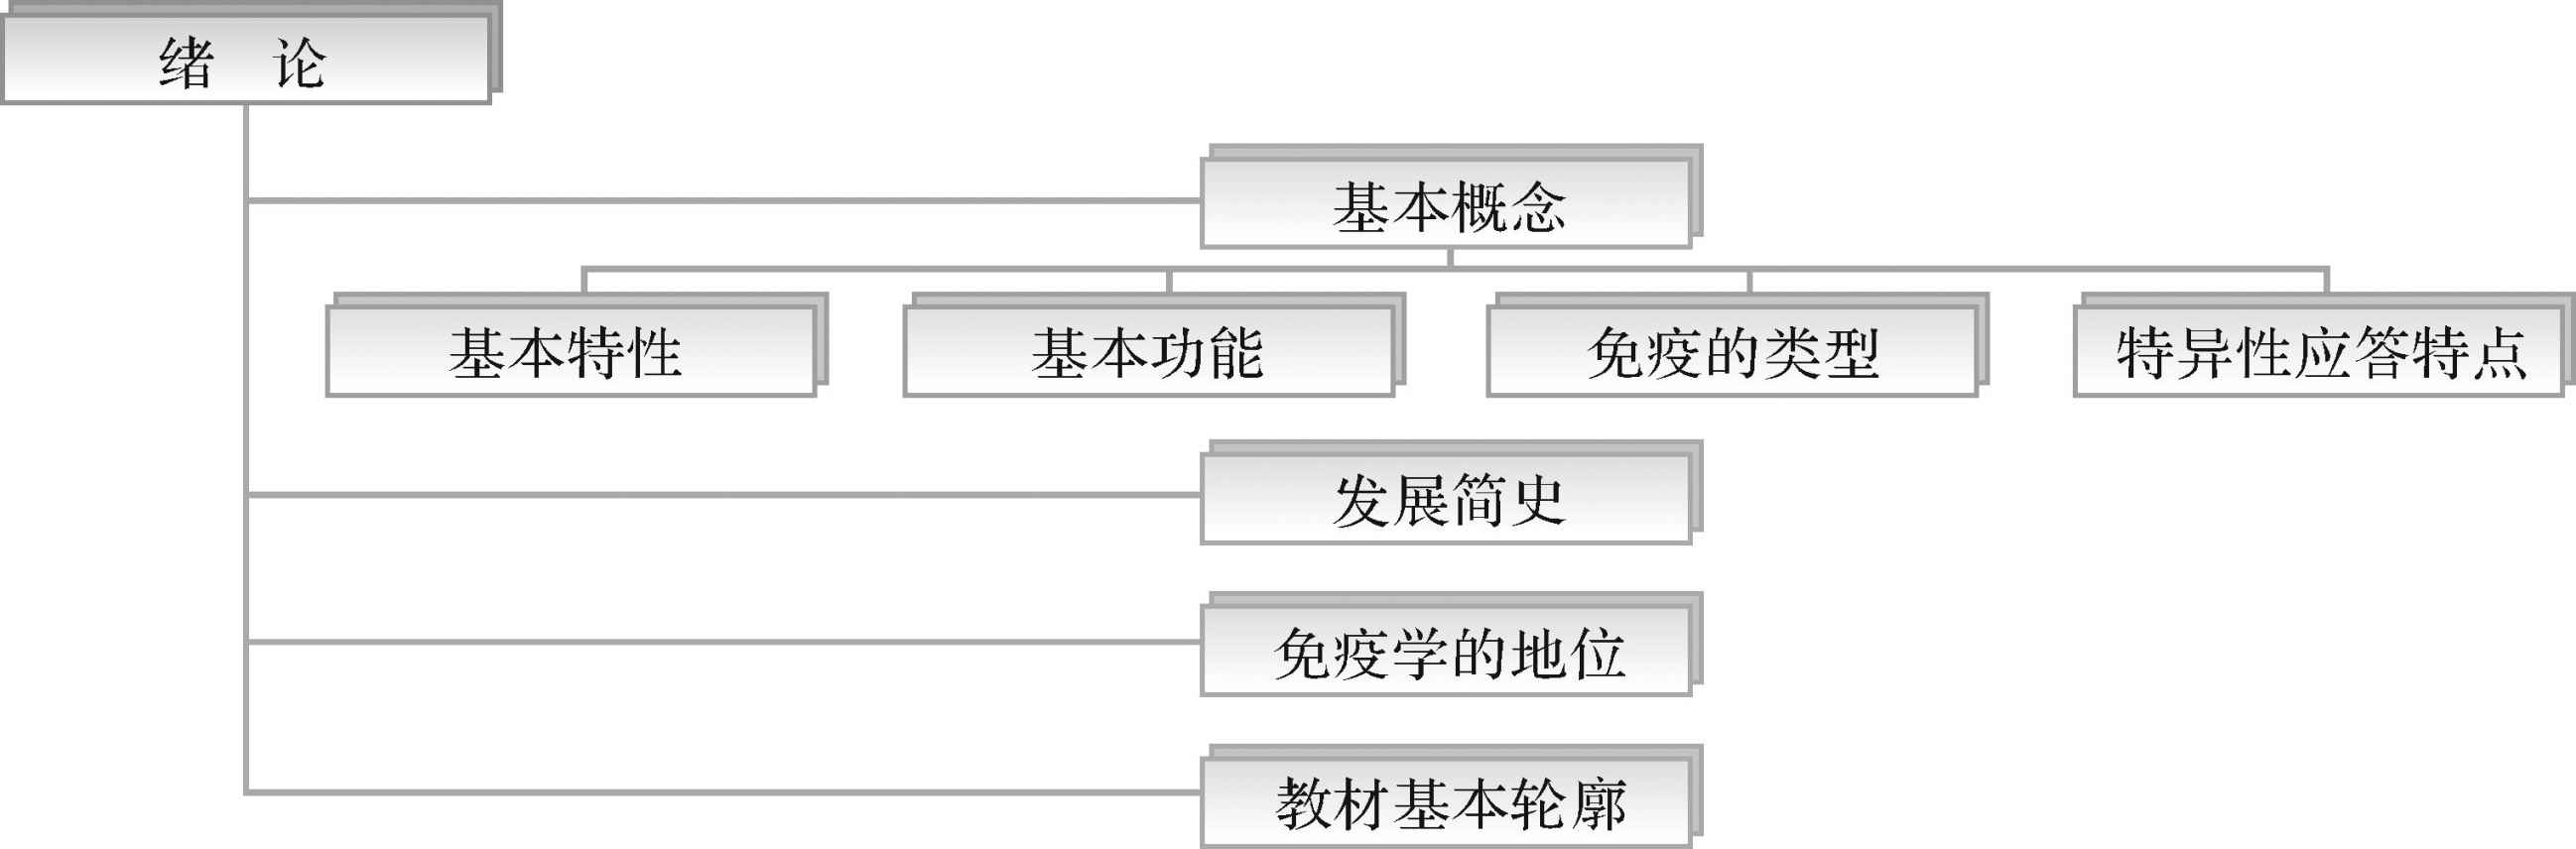
\includegraphics[width=0.6\textwidth]{./images/Image00007.jpg}
\end{center}
{\textbf 【课前思考】}

我们机体被各种病原体包围,机体中的细胞又不断癌变,每天有成千上万的细胞衰变死亡,但机体一般仍处于健康状态,为何?有外伤时,机体要化脓、发炎,而且仍有可能再次发炎,但得过某种传染病后一般不易再得同种传染病,为何?

{\textbf 【本章重点】}

1.免疫的基本概念、特性、功能;

2.免疫的类型。

{\textbf 【教学目标】}

1.掌握免疫的基本概念、特性、功能、类型;

2.熟悉免疫应答的类型;

3.了解免疫学发展简史,免疫学在生命科学中的地位。

\section{基本概念}

对免疫的认识源于人类对传染性疾病的抵御能力。“免疫(immunity)”一词即源于拉丁文immunitas,其本意是免除税赋和差役,引入医学领域则指免除瘟疫(传染病)。通过人们百余年的科学实践,已极大拓宽了对免疫的认识,现代免疫学将“免疫”的概念定义为:是机体识别“自己”与“非己”抗原、维持机体内外环境平衡的一种生理学反应。换言之,机体识别非己抗原,对其产生免疫应答并清除之;正常机体对自身组织抗原成分则不产生免疫应答,即维持耐受。


\subsection{免疫的基本特性}

1.识别自身和非自身。

2.特异性:能识别非自身物质间的微小差异,如同分异构体、旋光性等。

3.免疫记忆:有初次应答、再次应答。再次应答产生的抗体更多、更快,反应更强烈。如:传染病康复后或疫苗免疫后,能获得长期免疫力。


\subsection{免疫的基本功能}

免疫功能如同一把双刃剑,其对机体的影响具有双重性。正常情况下,免疫功能使机体内环境得以维持稳定,具有保护性作用;异常情况下,免疫功能可能导致某些病理过程的发生和发展。机体免疫系统通过对“自己”或“非己”物质的识别及应答(图\ref{fig1-1}),主要发挥如下三种功能:

1.免疫防御(immune
defence) 即抗感染免疫,主要指机体针对外来抗原(如微生物及其毒素)的免疫保护作用。在异常情况下,此类功能也可能对机体产生不利影响,表现为:若应答过强或持续时间过长,则在清除致病微生物的同时,也可能导致组织损伤和功能异常,即发生超敏反应;若应答过低或缺失,可发生免疫缺陷病。

2.免疫自稳(immune
homeostasis) 免疫细胞会把身体内的废物清除出体外,这些废物有敌人的尸体、老化死去的细胞、外来的杂质等,我们流出的汗与吐出的痰即属此类。该机制若发生异常,可能使机体对“自己”或“非己”抗原的应答出现紊乱,从而导致自身免疫病的发生。

3.免疫监视(immune
surveillance) 由于各种体内外因素的影响,正常个体的组织细胞不断发生畸变和突变。机体免疫系统可识别此类异常细胞并将其清除,此为免疫监视。若该功能发生异常,可能导致肿瘤的发生或持续的病毒感染(表\ref{tab1-1})。

\begin{figure}[!htbp]
 \centering
 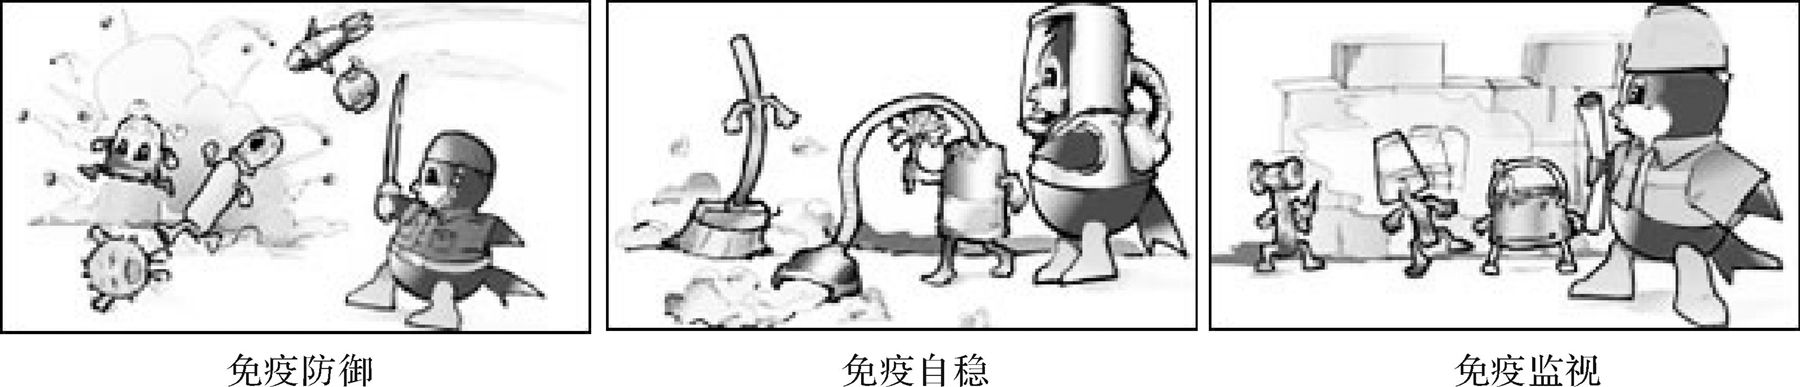
\includegraphics[width=0.8\textwidth]{./images/Image00008.jpg}
 \caption{免疫的基本功能}
 \label{fig1-1}
  \end{figure} 

\begin{longtable}[]{@{}lll@{}}
\caption{免疫功能的正常与异常表现}
\label{tab1-1}\\
\toprule
功能 & 正常表现 & 异常表现\tabularnewline
\midrule
\endhead
免疫防御 & 清除病原微生物(抗感染免疫) &
过强:超敏反应过弱:免疫缺陷病(慢性感染)\tabularnewline
免疫稳定 & 对自身组织成分耐受(消除损伤或衰老细胞) &
过强:自身免疫性疾病\tabularnewline
免疫监视 & 清除突变或癌变细胞(抗肿瘤免疫) &
过弱:肿瘤发生(病毒持续感染)\tabularnewline
\bottomrule
\end{longtable}


\subsection{免疫的类型}

机体的“免疫”可分为天然免疫和获得性免疫两类。

1.天然免疫

天然免疫(innate
immunity)即固有免疫,是机体抵御微生物侵袭的第一道防线。其特点是:个体出生时即具备,作用范围广,并非针对特定抗原,故亦称为非特异性免疫(nonspecific
immunity)。此类免疫的主要机制为:皮肤、黏膜及其分泌的抑菌/杀菌物质的屏障效应;体内多种非特异性免疫效应细胞和效应分子的生物学作用。

2.获得性免疫

获得性免疫(acquired
immunity)即适应性(adaptive)免疫,乃个体接触特定抗原而产生,仅针对该特定抗原而发生反应,故亦称为特异性免疫(specific
immunity)。此类免疫主要由能够特异性识别抗原的免疫细胞(即T淋巴细胞和B淋巴细胞)所承担,其所产生的效应在机体抗感染和其他免疫学机制中发挥主导作用,天然免疫和获得性免疫的比较见表\ref{tab1-2}。特异性免疫应答的基本过程是:T淋巴细胞和B淋巴细胞特异性识别抗原并被活化,继而分化为效应细胞,最终介导细胞免疫或体液免疫效应(如清除病原体等)。

\begin{longtable}[]{@{}ll@{}}
\caption{天然免疫和获得性免疫的比较}
\label{tab1-2}\\
\toprule
天然免疫(非特异性免疫) & 获得性免疫(特异性免疫)\tabularnewline
\midrule
\endhead
抗原非依赖性 & 抗原依赖性\tabularnewline
立即达到最大反应 & 达到最大反应时间滞后(96小时后)\tabularnewline
无抗原特异性 & 抗原特异性\tabularnewline
无免疫记忆 & 产生免疫记忆\tabularnewline
\bottomrule
\end{longtable}


\subsection{特异性免疫应答的特点}

特异性免疫应答(简称为免疫应答)是由抗原刺激机体免疫系统所致,包括抗原特异性淋巴细胞对抗原的识别、活化、增殖、分化及产生免疫效应的全过程。免疫应答具有如下特点:

1.特异性

获得性免疫的特异性表现为:一方面,特定的免疫细胞克隆仅能识别特定抗原;另一方面,应答中所形成的效应细胞和效应分子(抗体)仅能与诱导其产生的特定抗原发生反应。

2.记忆性

获得性免疫的记忆性表现为:参与特异性免疫的T淋巴细胞和B淋巴细胞均具有保存抗原信息的功能。它们初次接触特定抗原并产生应答后,可形成特异性记忆细胞,以后再次接触相同抗原刺激时,可迅速被激活并大量扩增,产生更强的再次应答。获得性免疫的记忆性可由图\ref{fig1-2}表示。

3.耐受性

免疫细胞接受抗原刺激后,既可产生针对特定抗原的特异性应答,也可表现为针对特定抗原的特异性不应答,后者即为免疫耐受。机体对自身组织成分的耐受遭破坏或对致病抗原(如肿瘤抗原或病毒抗原)产生耐受,均可导致某些病理过程的发生。

\begin{figure}[!htbp]
 \centering
 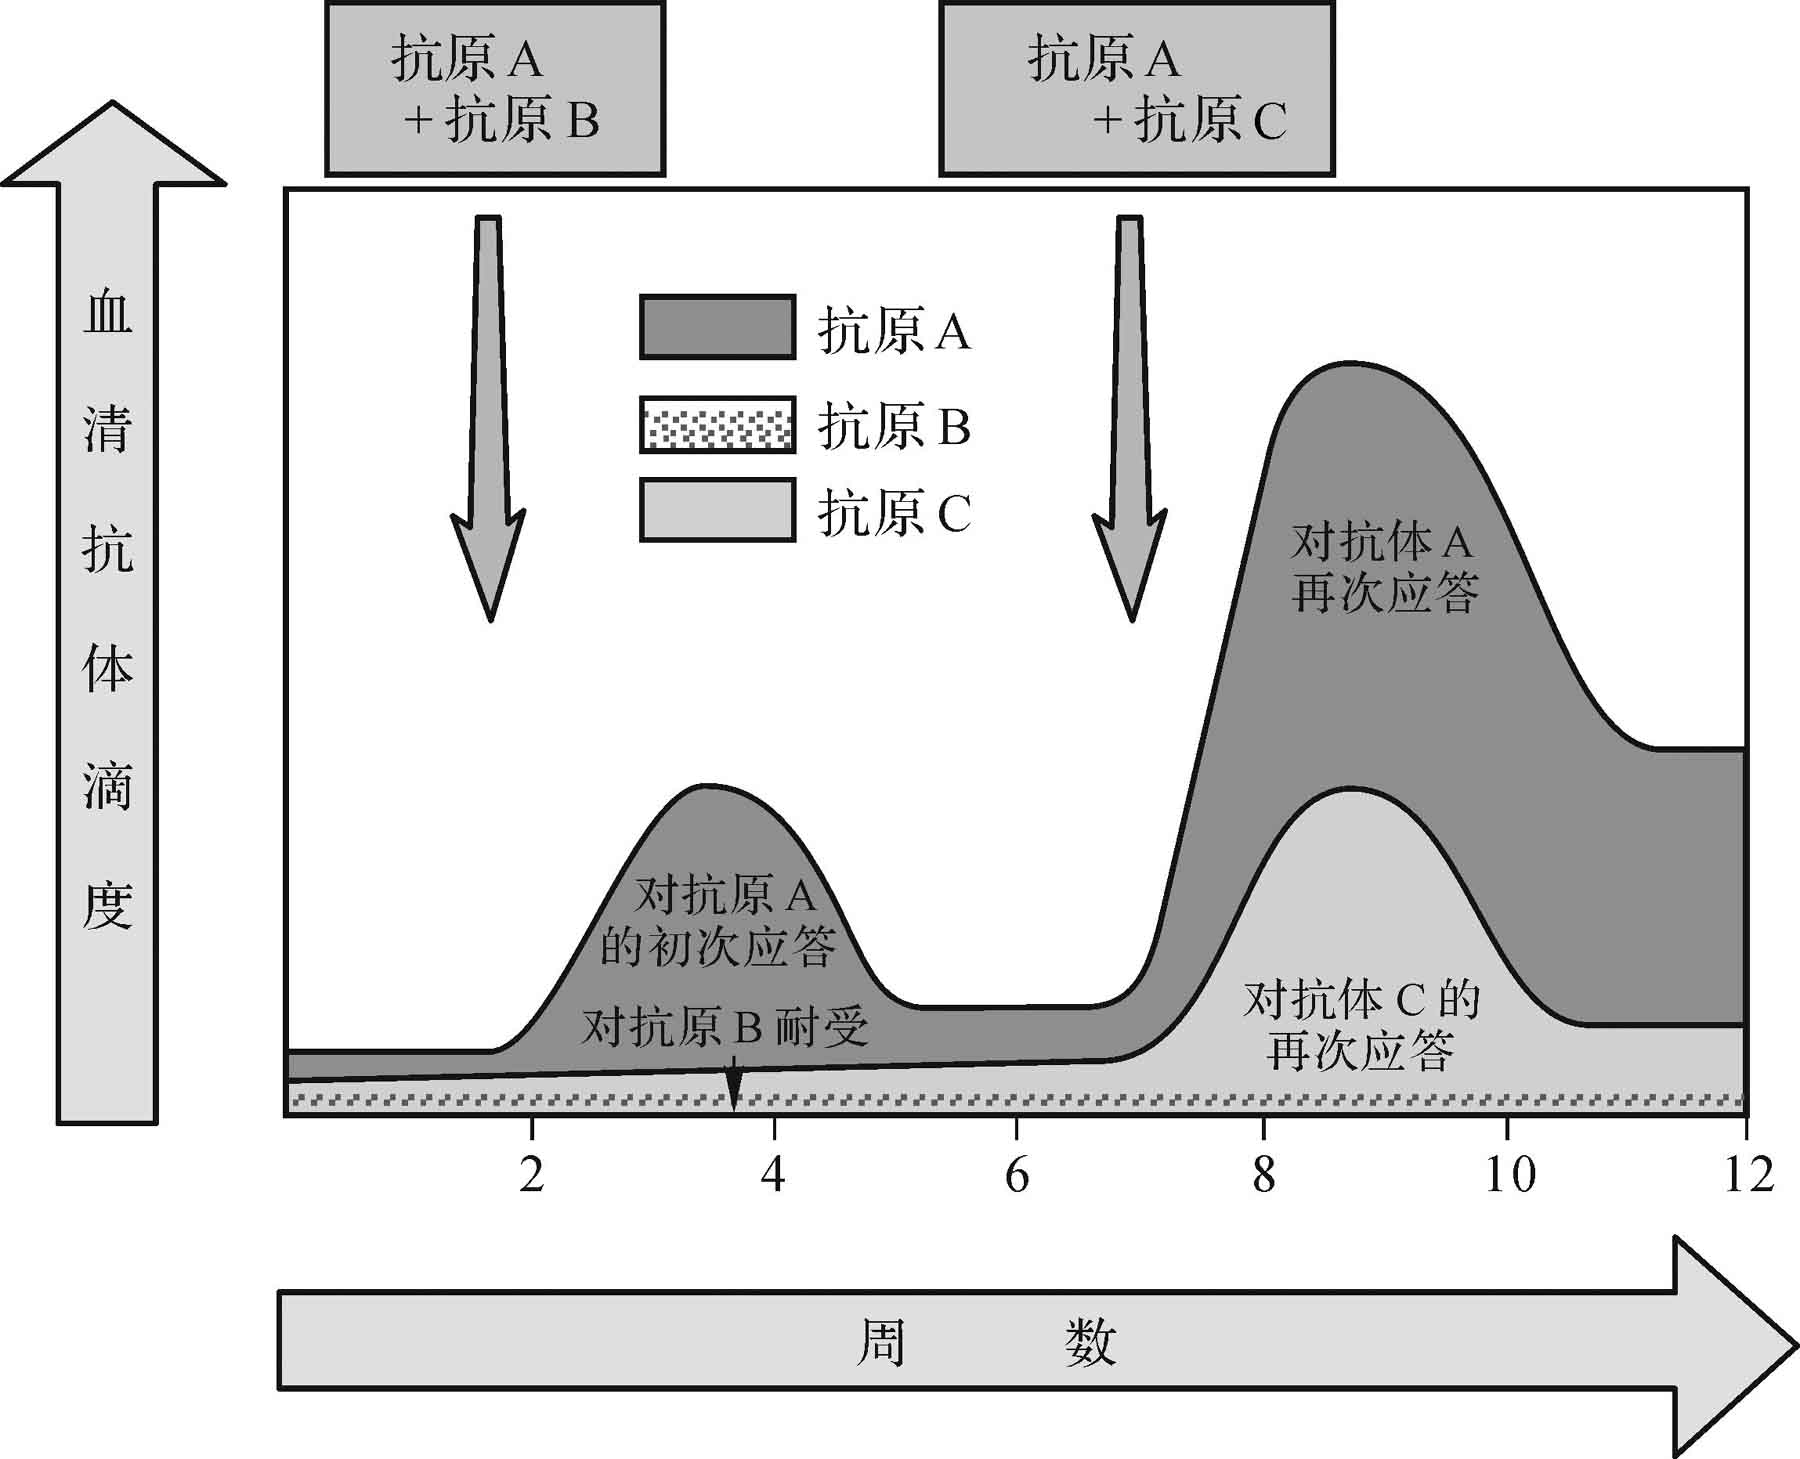
\includegraphics[scale=1.1]{./images/Image00009.jpg}
 \caption{免疫应答的记忆性}
 \label{fig1-2}
  \end{figure} 

\section{免疫学发展简史}

免疫学建立至今已有数百年历史,根据其特点可分为若干时期。


\subsection{经验免疫学时期(17世纪~19世纪)}

早在16~17世纪(明代)我国史书已有正式记载:将沾有疱浆的天花患者衣服给正常儿童穿戴,或将天花愈合后的局部痂皮磨碎成细粉,经鼻给正常儿童吸入,可预防天花。这种应用人痘苗预防疾病的医学实践,可视为人类认识机体免疫力的开端,也是我国传统医学对人类的伟大贡献。18世纪初,我国应用痘苗预防天花的方法传至国外,并为以后牛痘苗和减毒疫苗的发明提供了宝贵经验。至18世纪末,英国医生Edward
Jenner首先观察到挤奶女工感染牛痘后不易患天花,继而通过人体实验确认接种牛痘苗可预防天花。他把接种牛痘称为
“Vaccination”
(拉丁文Vacca为牛),于1798年发表了相关论文。接种牛痘苗乃划时代的发明,为人类传染病的预防开创了人工免疫的先声(图\ref{fig1-3})。在此阶段,人们对免疫学现象主要为感性认识,故称为经验免疫学时期。1978
年世界卫生组织宣布人类消灭了天花。

\begin{figure}[!htbp]
 \centering
 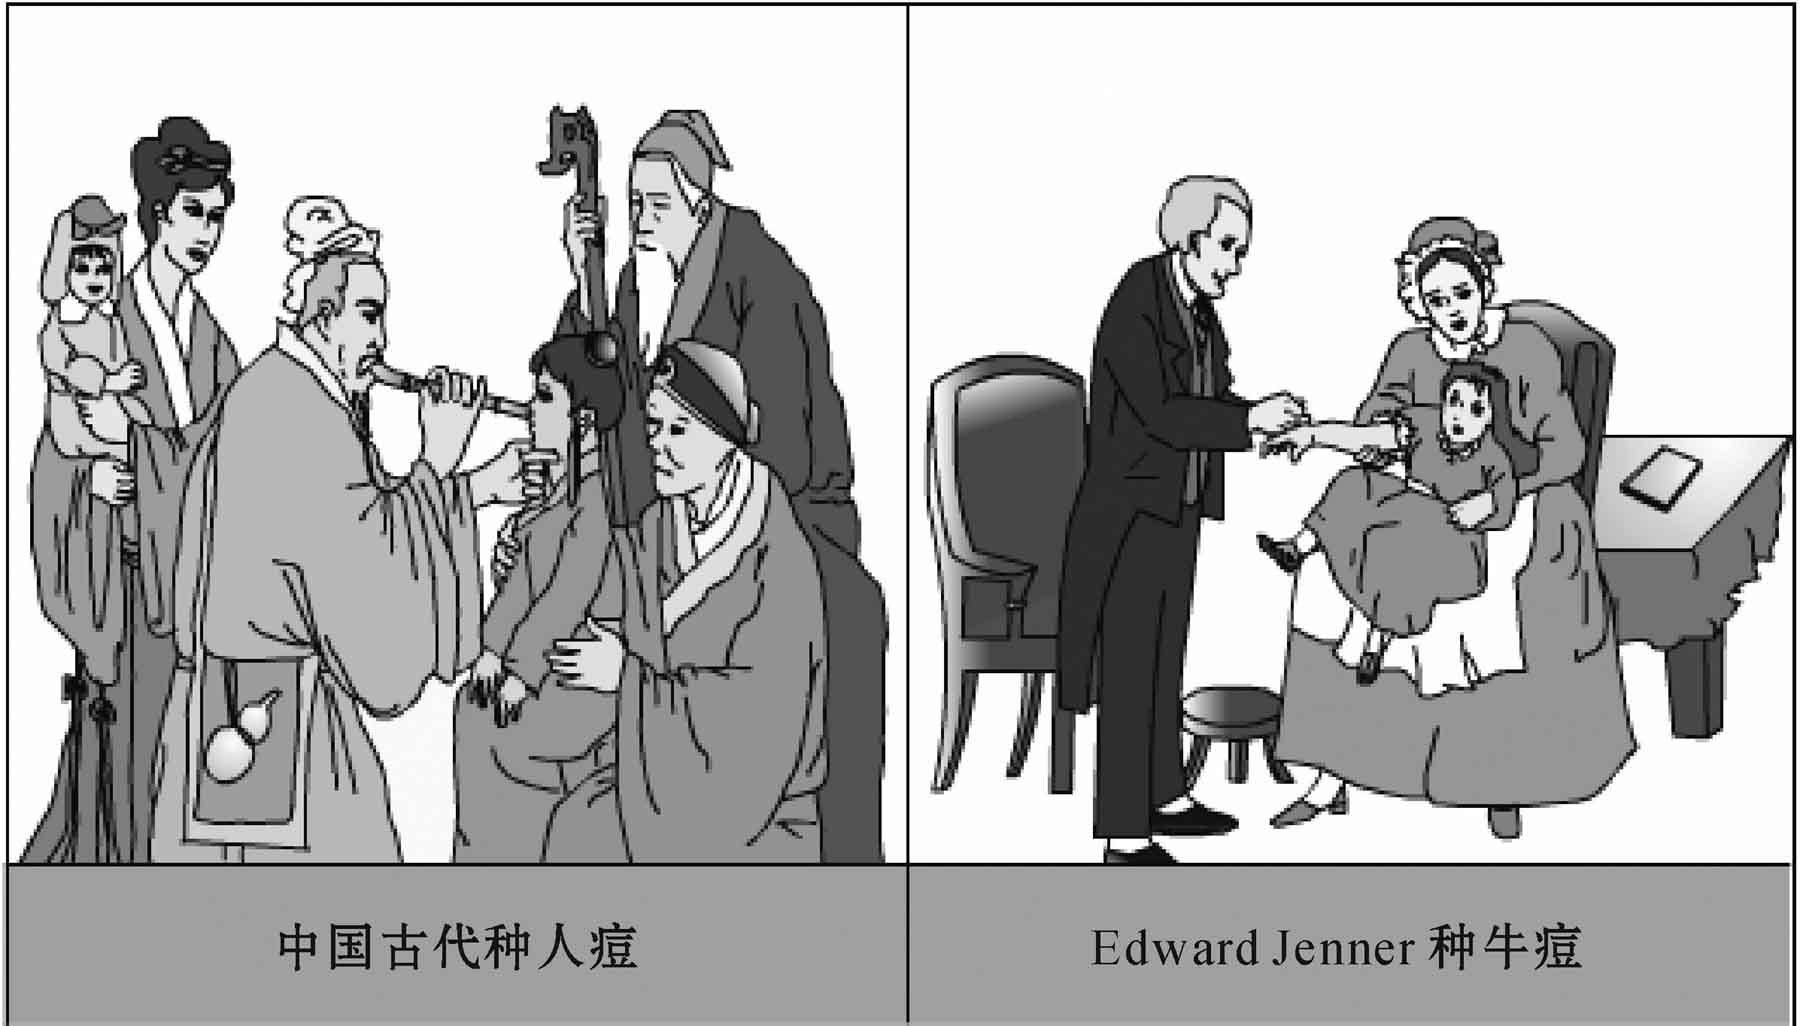
\includegraphics{./images/Image00010.jpg}
 \caption{种牛痘}
 \label{fig1-3}
  \end{figure} 


\subsection{经典免疫学时期(19世纪中叶~20世纪中叶)}

自19世纪中叶始,L.Pastuer等(图\ref{fig1-4})先后发现多种病原菌,极大促进了疫苗的发展和使用。人们开始尝试应用灭活及减毒的病原体制成多种疫苗,分别预防不同传染性疾病。免疫学在此期的发展与微生物学密切相关,并成为微生物学的一个分支。此时,人们对“免疫”的认识已不仅限于单纯地观察人体现象,而是进入了科学实验时期。

\begin{figure}[!htbp]
 \centering
 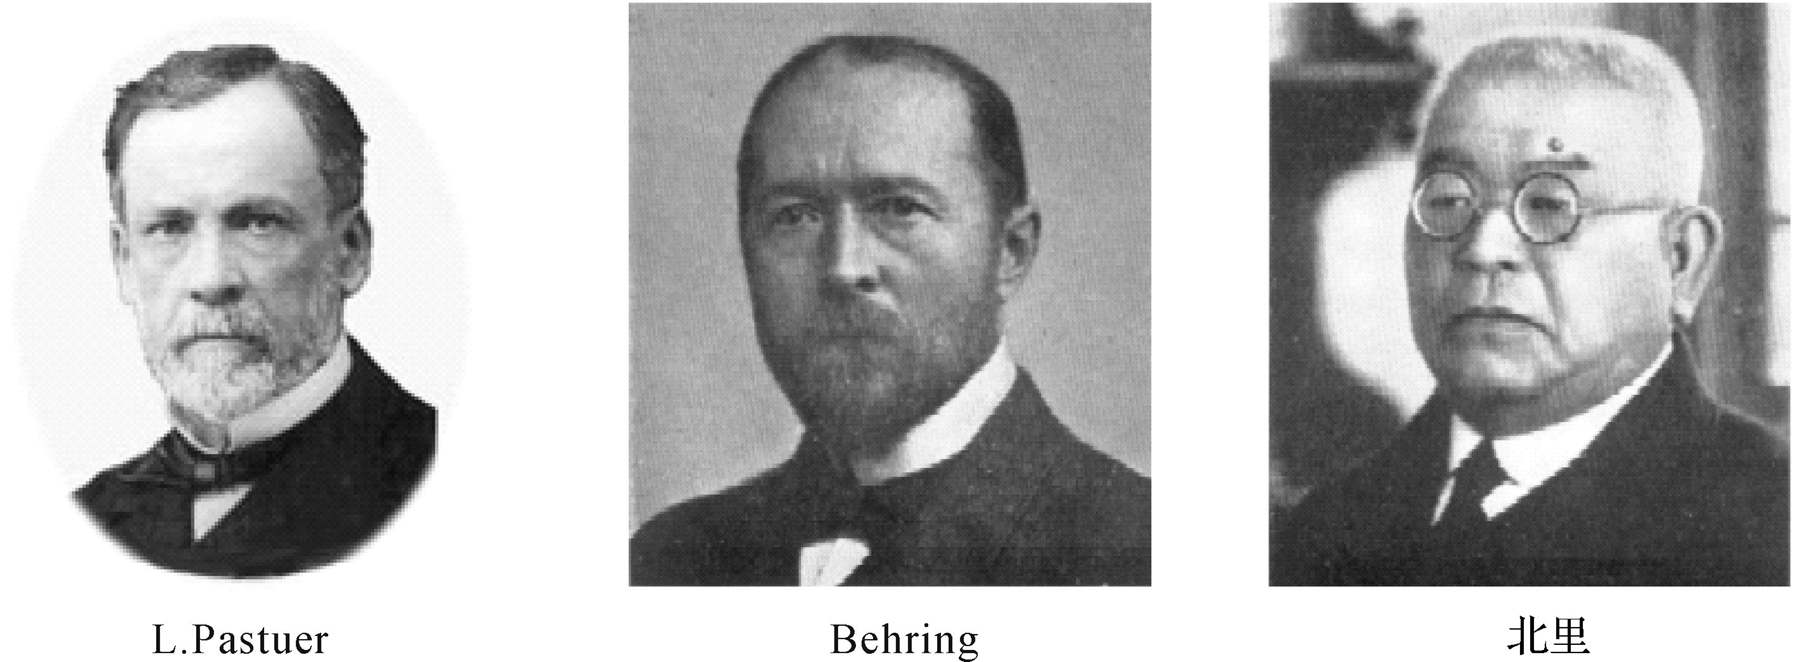
\includegraphics[width=.7\textwidth]{./images/Image00011.jpg}
 \caption{免疫学家}
 \label{fig1-4}
  \end{figure} 

(一)抗体的发现

德国学者Behring和日本学者Kitasato(图\ref{fig1-4})于1890年在Koch研究所应用白喉外毒素给动物免疫,发现在其血清中有一种能中和外毒素的物质,称为抗毒素。将这种免疫血清转移给正常动物也有中和外毒素的作用。这种被动免疫法很快应用于临床治疗。Behring于1891年应用来自动物的免疫血清成功地治疗了一个白喉患者,这是第一个被动免疫治疗的病例。为此,他于1902年获得了诺贝尔医学奖。

20世纪30年代,Tiselius和Kabat用电泳鉴定,证明Ab是γ-球蛋白。动物在免疫后,血清中γ-球蛋白显著增高,此部分有Ab活性,从而可将Ab从血清中分离出来,Ab主要存在于γ-球蛋白。抗体是四肽链结构。1959年,Porter
和Edelman对抗体结构进行研究证明是由四条对称的多肽链构成单体包括两条相同的分子量较大的重链和两条相同的分子量较小的轻链构成,如图\ref{fig1-5}所示。

\begin{figure}[!htbp]
 \centering
 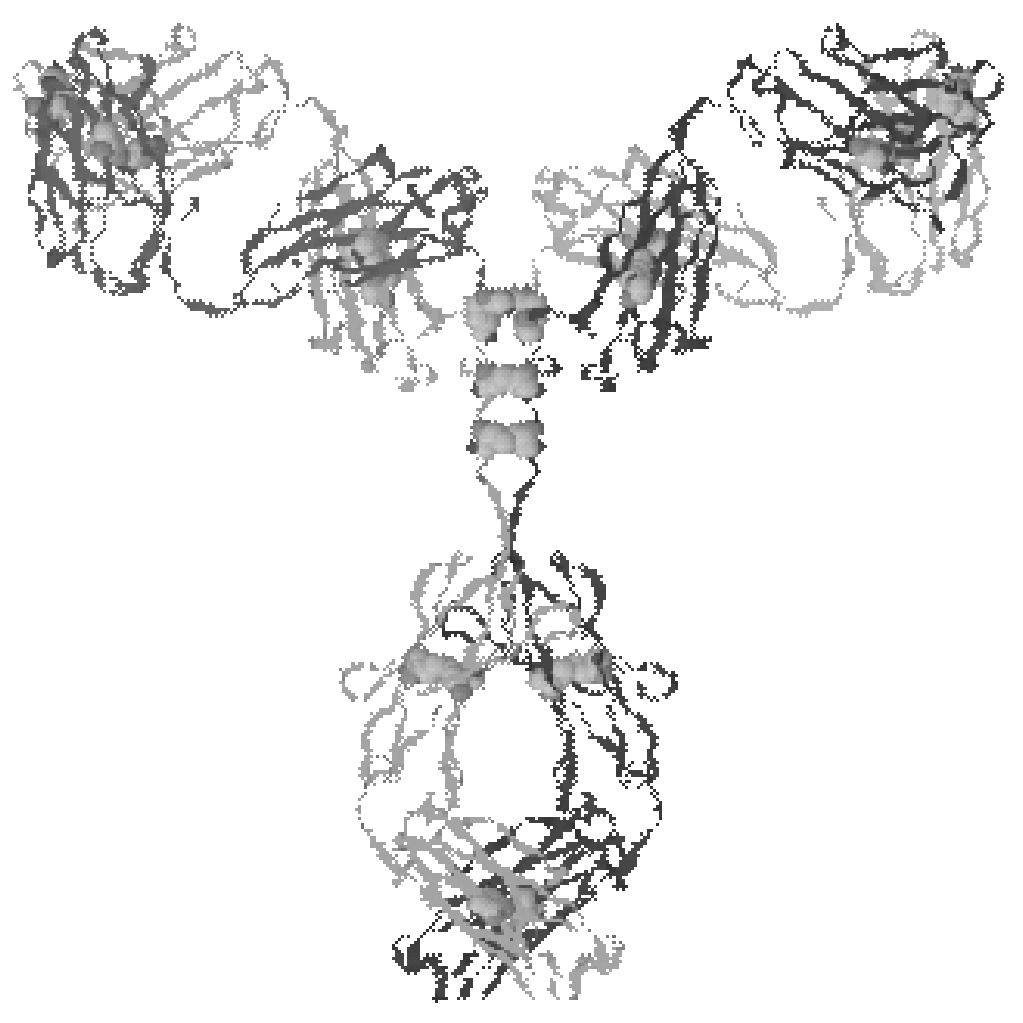
\includegraphics[scale=1.2]{./images/Image00012.jpg}
 \caption{抗体的结构}
 \label{fig1-5}
  \end{figure} 

\begin{figure}[!htbp]
 \centering
 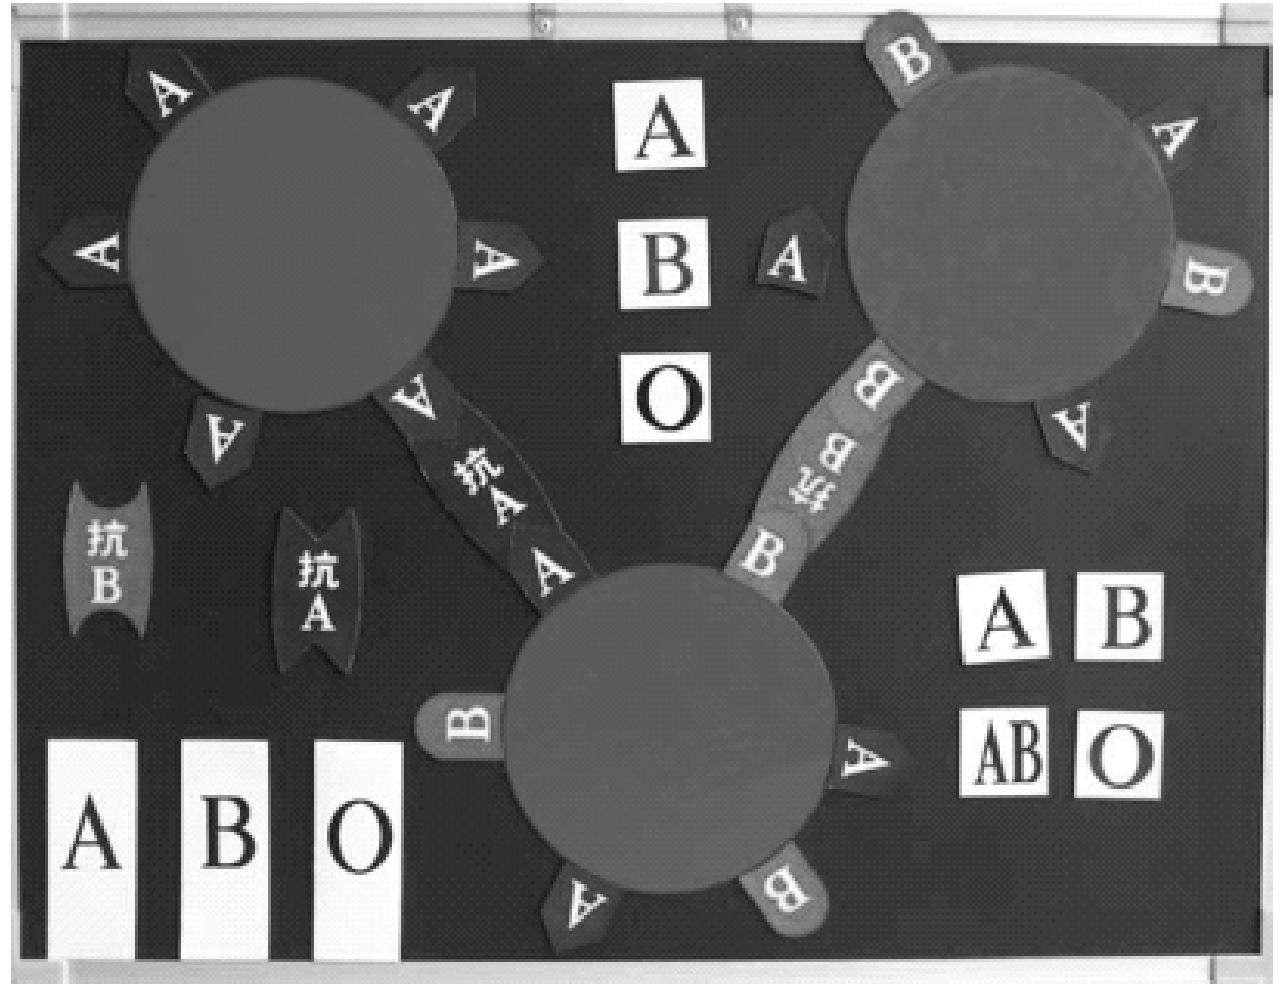
\includegraphics{./images/Image00013.jpg}
 \caption{ABO血型}
 \label{fig1-6}
  \end{figure} 

(二)抗原的结构与抗原特异性

20世纪初开始,Landsteiner以芳香族有机化学分子耦联到蛋白质分子上免疫动物,研究芳香族分子的结构与活性基团的部位对产生的抗体特异性的影响,认识到决定抗原特异性的是很小的分子,它们的结构不同,使其抗原性不同。据此,Landsteiner发现人红细胞表面表达的糖蛋白中,其末端寡糖特点决定了它的抗原性,从而发现了ABO血型(图\ref{fig1-6}),避免了输血导致严重超敏反应的问题。

(三)超敏反应

早在20世纪初即发现:应用动物来源的Ab作临床治疗,能引起患者的血清病,严重者致休克。后来von
Pirguet证明在结核病患者进行结核菌素的皮肤划痕试验,能致局部显著的病理改变(图\ref{fig1-7})。他总结这类由免疫应答而致的疾病,称之为变态反应(allergy)。从而,揭示超敏的不适宜的免疫应答对机体有害的一面。

\begin{figure}[!htbp]
 \centering
 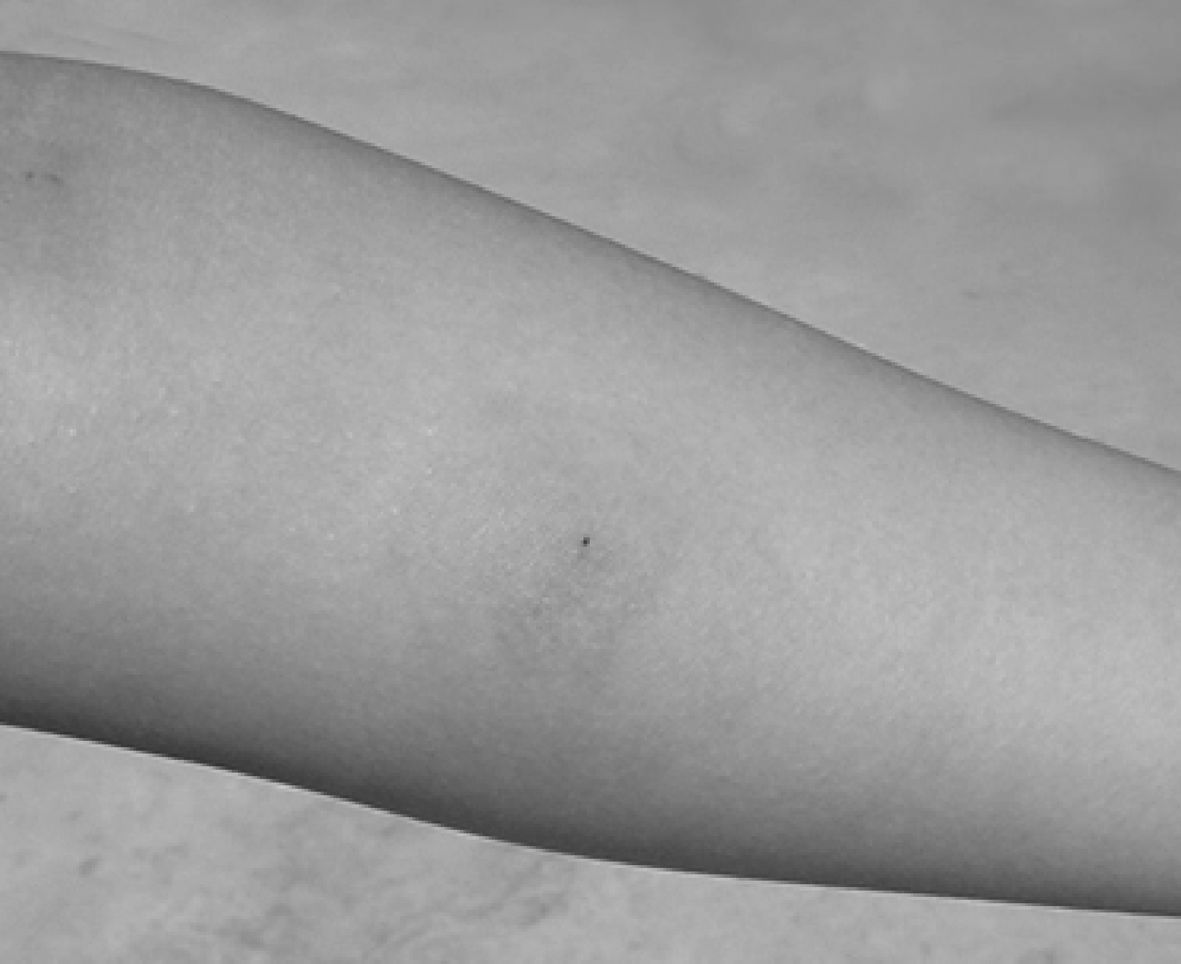
\includegraphics[width=0.5\textwidth]{./images/Image00014.jpg}
 \caption{超敏反应}
 \label{fig1-7}
  \end{figure} 

(四)免疫耐受的发现

1945年,Owen发现自异卵双生的两头小牛个体内有两种血型红细胞共存,称之为血型细胞镶嵌现象(图\ref{fig1-8})。这种不同血型细胞在彼此体内互不引起免疫反应,他把这种现象称为天然耐受。

1953年,Medawar等进一步用实验证实了此一免疫耐受现象(图\ref{fig1-9})。
\begin{figure}[!htbp]
    \centering
    \begin{minipage}[b]{0.45\textwidth} 
        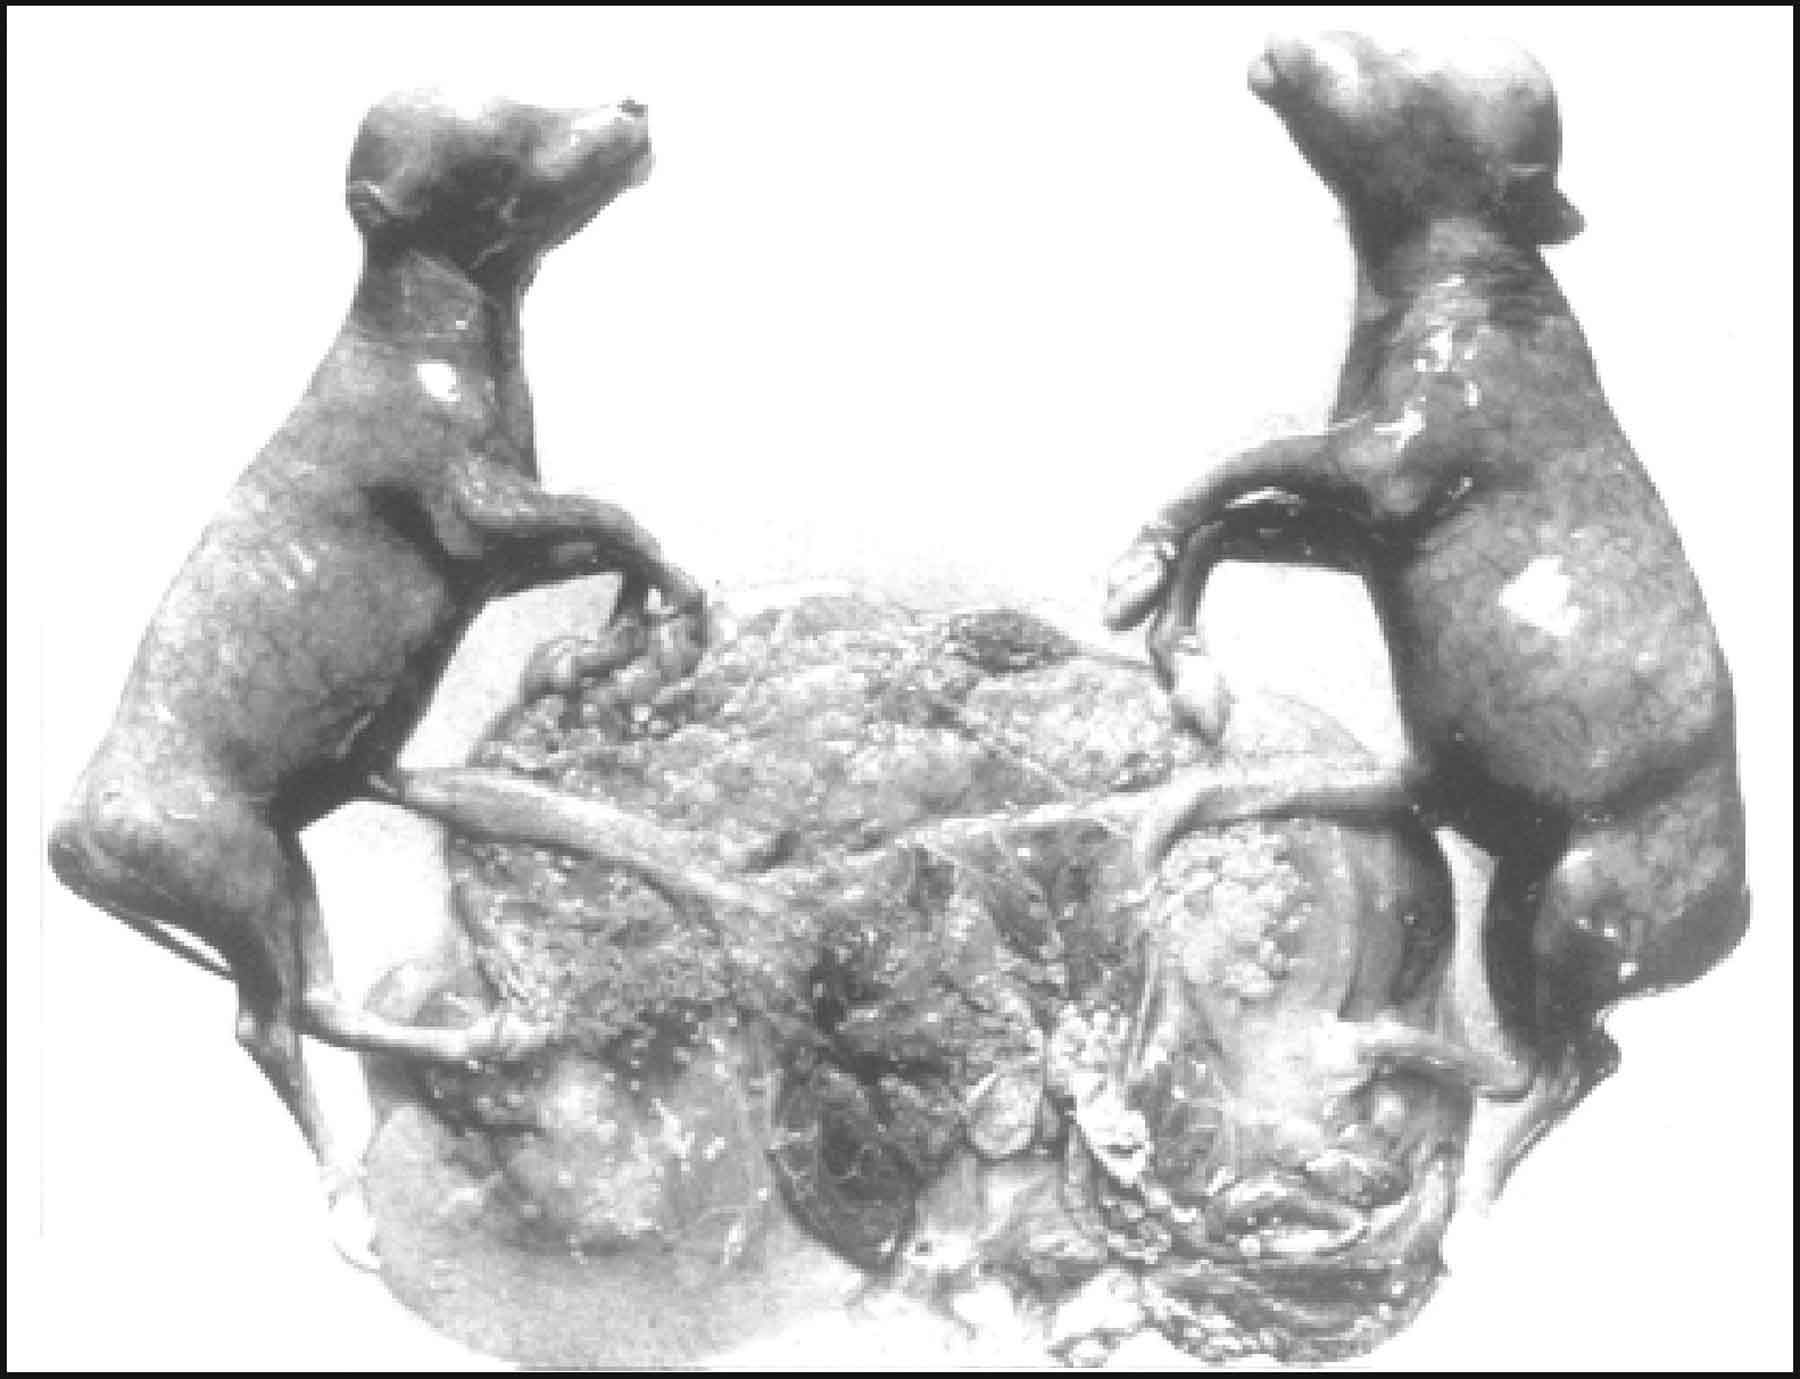
\includegraphics[height=0.2\textheight]{./images/Image00015.jpg}
        \caption{血型细胞镶嵌现象}
        \label{fig1-8}
    \end{minipage}
%	\end{figure} 
	%\FloatBarrier
%\begin{figure}[!htbp]
%    \centering
\hspace{0.04\textwidth}%
\begin{minipage}[b]{0.45\textwidth} 
    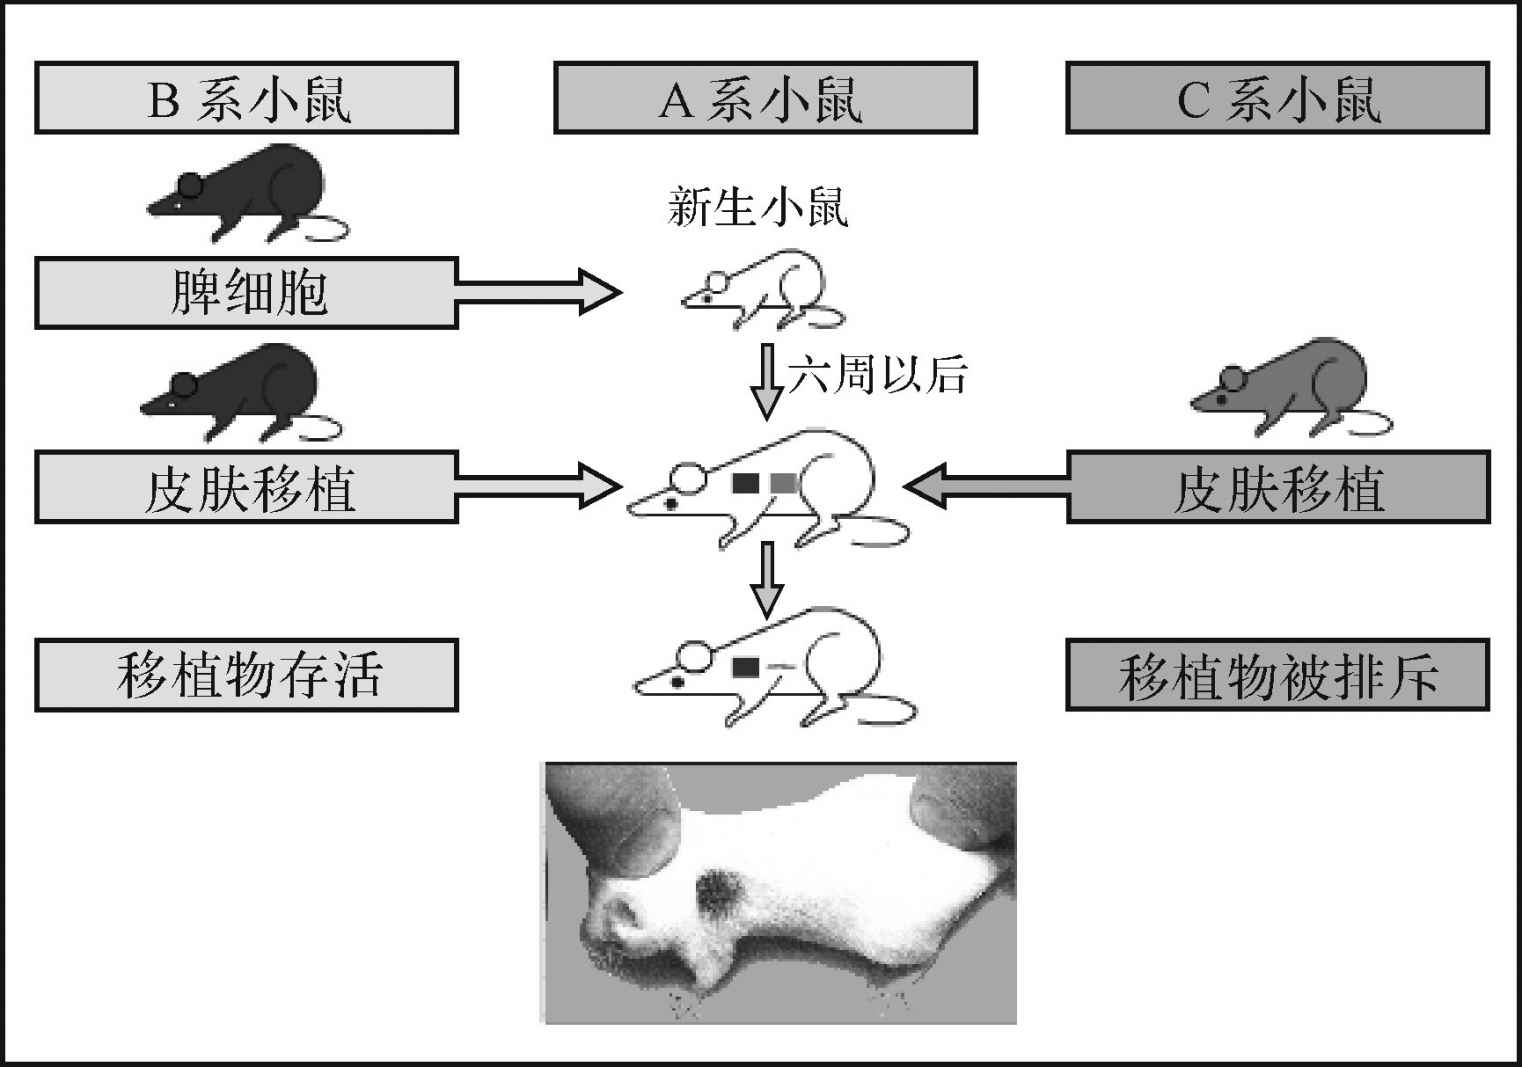
\includegraphics[height=0.2\textheight]{./images/Image00016.jpg}
 \caption{免疫耐受}
 \label{fig1-9}
\end{minipage}
\end{figure} 

(五)免疫应答机制的研究

关于机体免疫机制的研究和探讨,出现了两派学说:

1.细胞免疫:俄国梅契尼可,发现白细胞有吞噬功能,能吞噬和清除各种病原微生物。

2.体液免疫:德国欧立希,体液中产生的抗体,能清除各种病原微生物。

(六)1959年Burnet学说及其对免疫学发展的推动作用------克隆选择学说

F.M.Burnet在前人的研究基础上于1959年提出了克隆选择学说(图\ref{fig1-10}),为免疫生物学发展奠定了理论基础,使免疫学超越了传统的抗感染免疫,从而开启了现代免疫学新阶段。迄今50余年来,人们从整体、器官、细胞、分子和基因水平探讨免疫系统的结构与功能,并阐明基本免疫学现象的本质及其机制,在涉及免疫学基础理论和实践应用的各领域展开了深入而系统的研究,并不断取得突破性进展,对生物学和医学发展产生了深刻影响。至今,免疫学已发展为覆盖面极广的前沿学科,并成为现代生物医学的支柱学科之一。

\begin{figure}[!htbp]
 \centering
 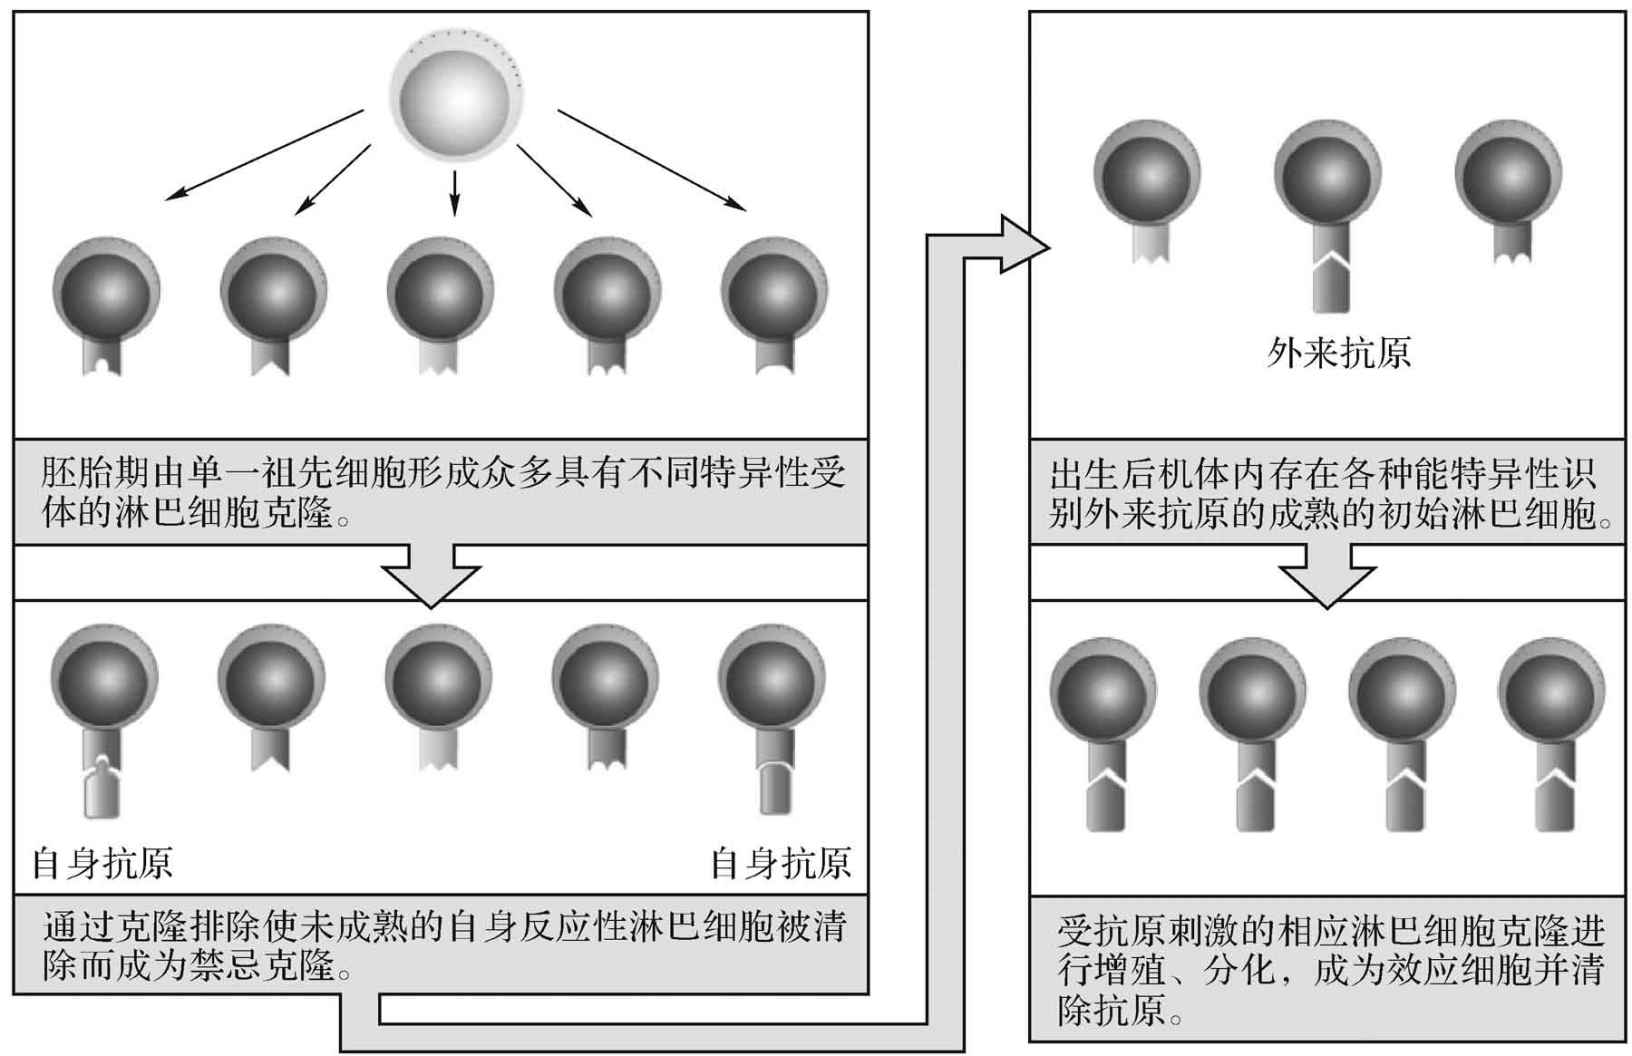
\includegraphics[width=0.7\textwidth]{./images/Image00017.jpg}
 \caption{克隆选择学说示意图}
 \label{fig1-10}
  \end{figure} 

克隆选择学说的要点有四点:

(1)
体内存在多种针对各种抗原的免疫细胞克隆,其表面有识别抗原的受体(一个克隆针对一种抗原)。

(2)
抗原进入机体内选择相应细胞克隆,使其活化、增殖、分化成抗体产生细胞或免疫效应细胞。

(3)胚胎期,某一免疫细胞克隆接触相应的抗原,如自身成分,则被排除或处于抑制状态,称为禁忌克隆,不能对自身抗原产生免疫应答而形成自身耐受。

(4)某些情况下,禁忌细胞株可以活化,对自身抗原发生免疫应答而形成自身免疫或自身免疫性疾病。


\subsection{现代免疫学时期(20世纪中叶至今)}

(一)抗原识别受体多样性的产生

1978年,发现抗体基因重排是B细胞抗原识别受体多样性的原因(图\ref{fig1-11})。

\begin{figure}[!htbp]
 \centering
 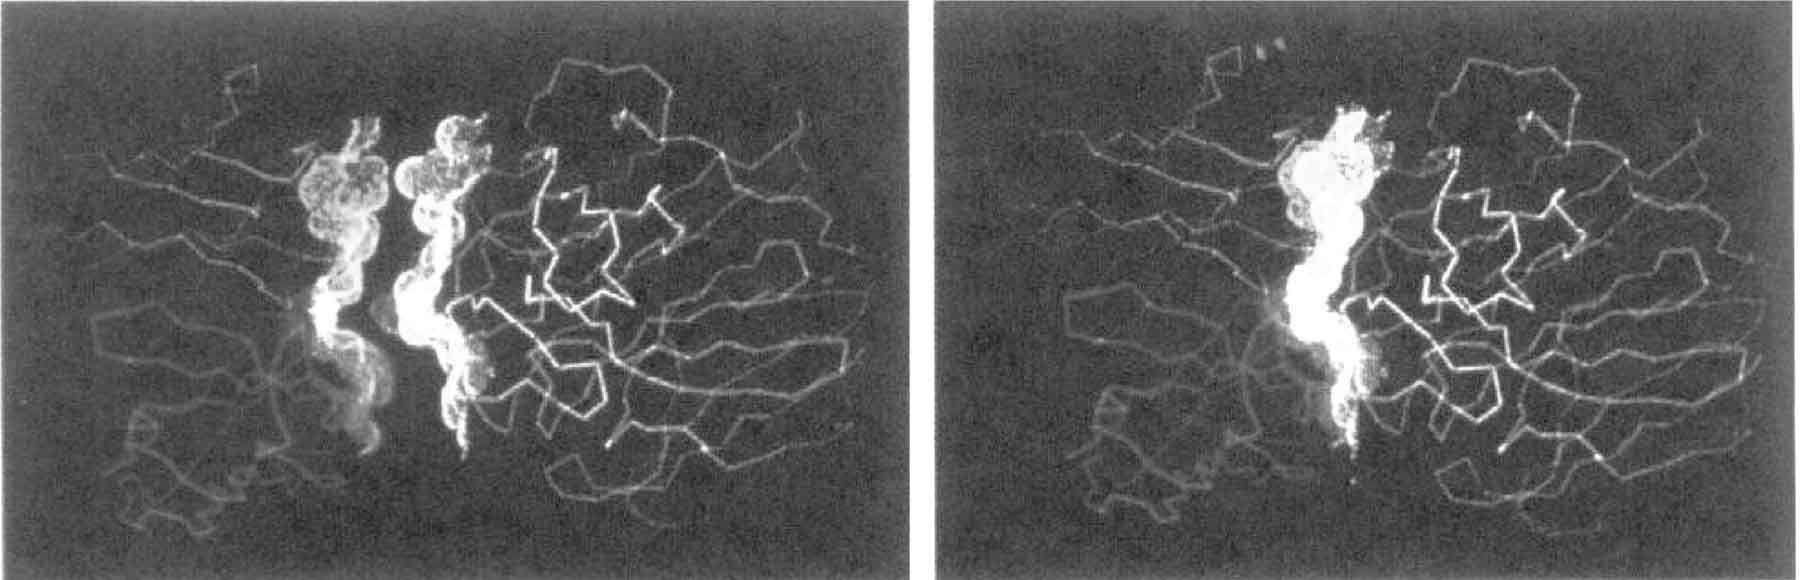
\includegraphics[scale=1.1]{./images/Image00018.jpg}
 \caption{抗原识别受体多样性}
 \label{fig1-11}
  \end{figure} 

(二)信号转导途径的发现

20世纪80年代,发现了T淋巴细胞识别抗原的MHC限制性;至90年代,发现T淋巴细胞活化需要双信号作用(图\ref{fig1-12})。

\begin{figure}[!htbp]
 \centering
 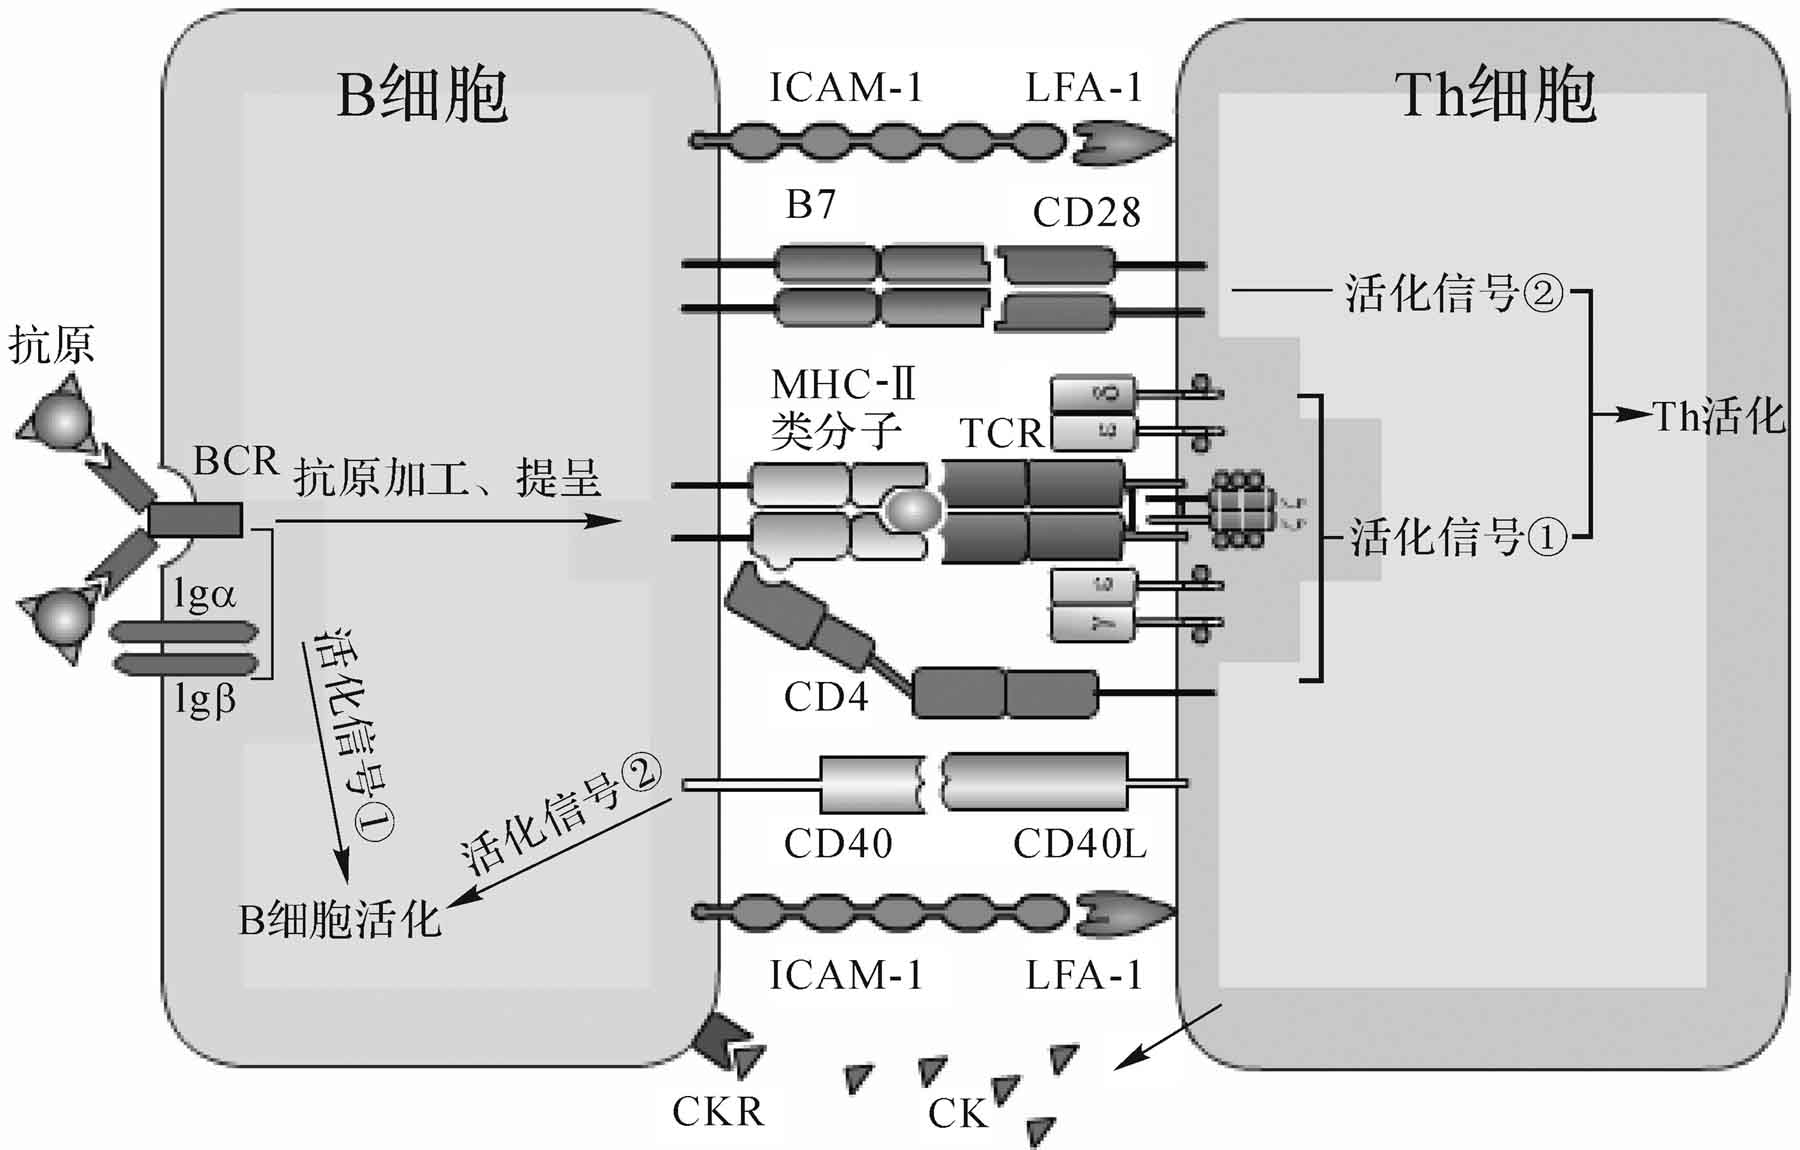
\includegraphics[scale=1.2]{./images/Image00019.jpg}
 \caption{细胞活化双信号}
 \label{fig1-12}
  \end{figure} 

\begin{figure}[!htbp]
 \centering
 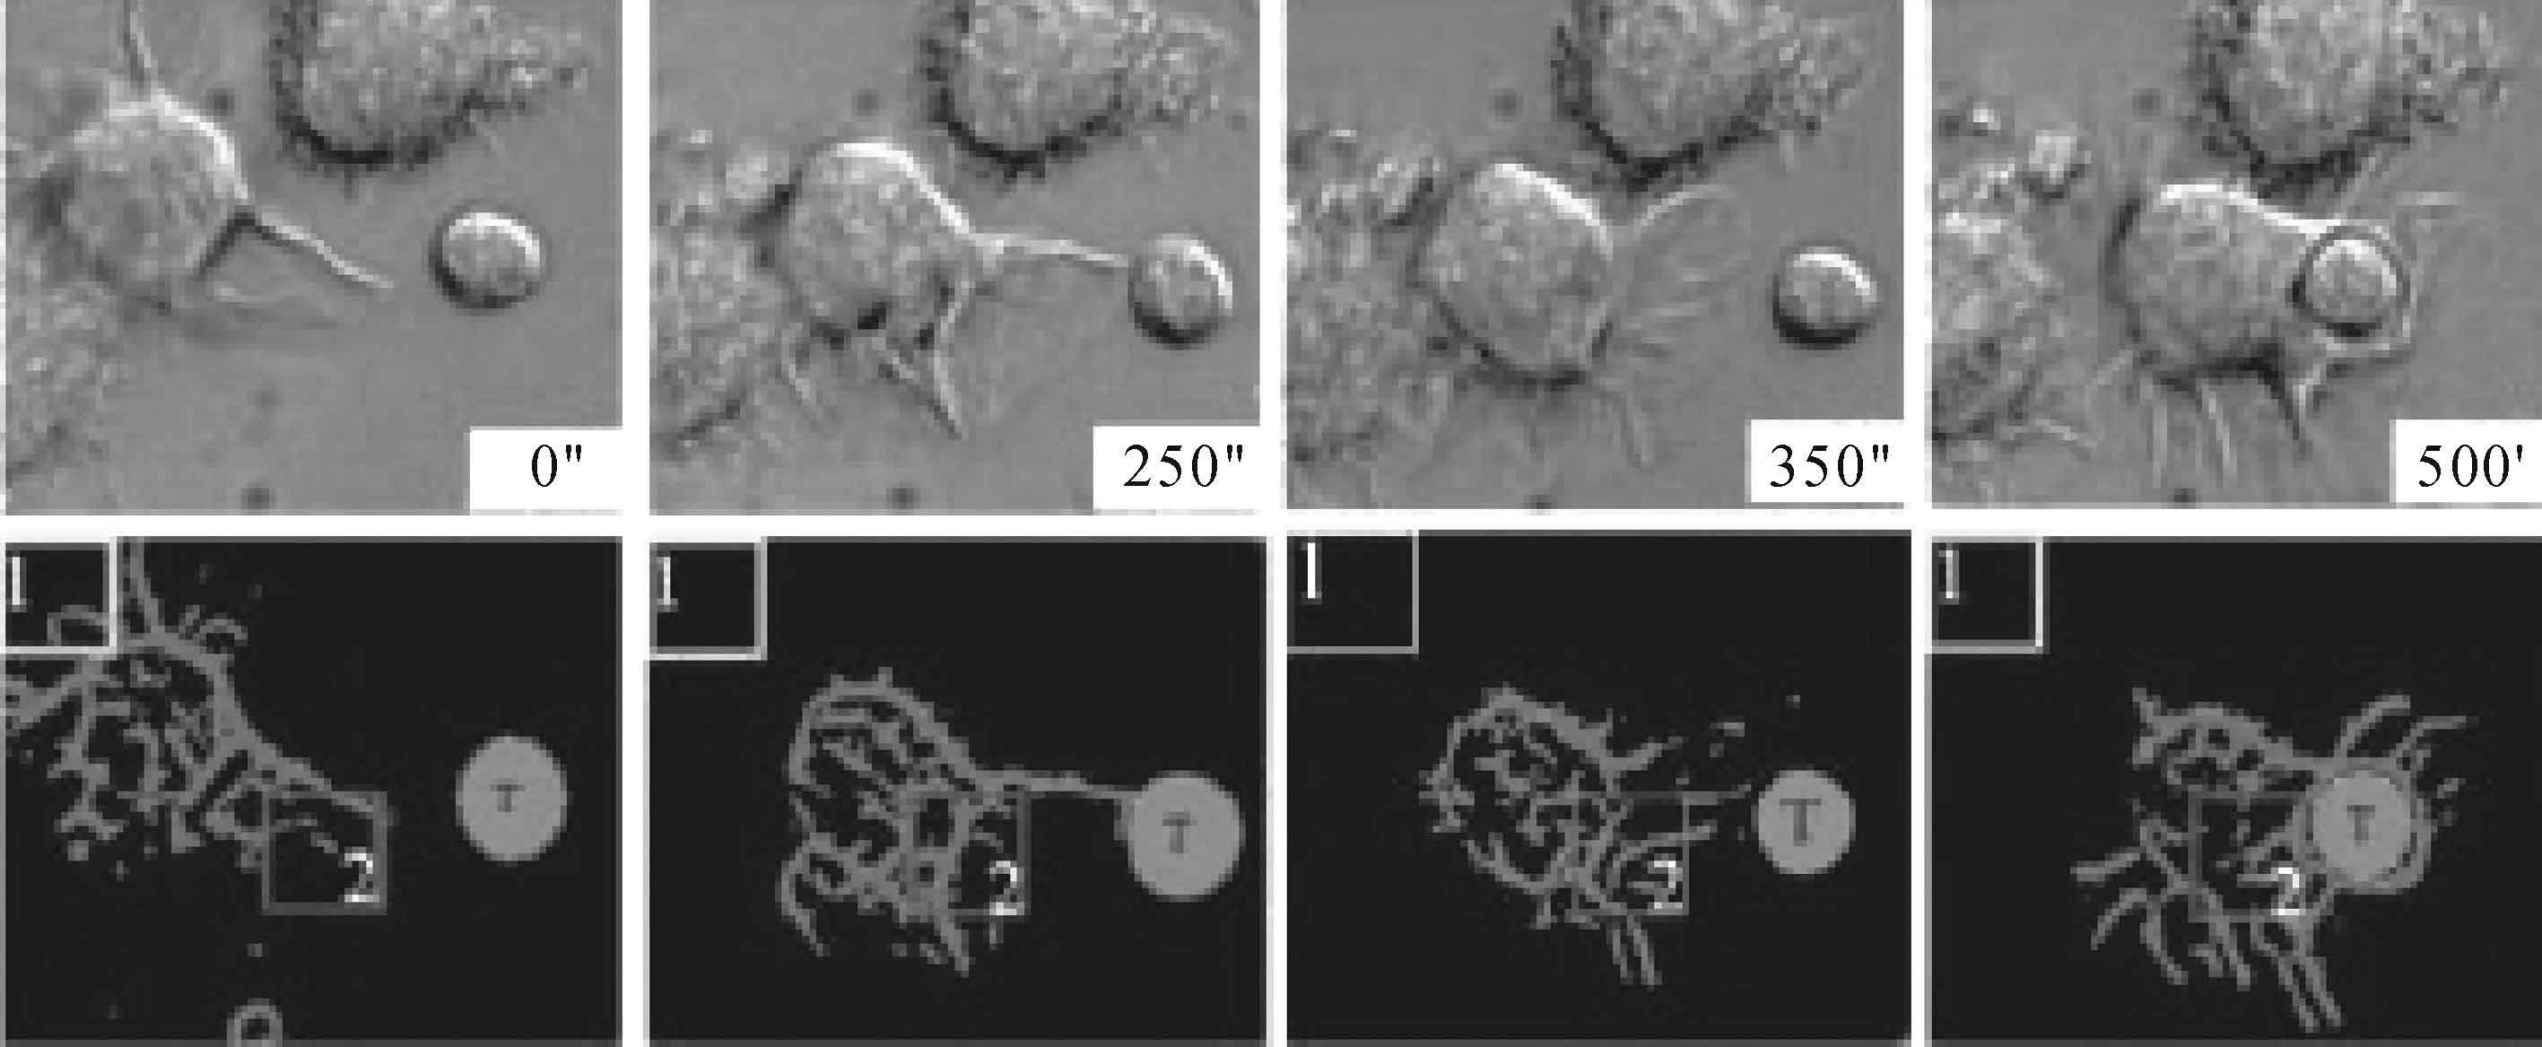
\includegraphics{./images/Image00020.jpg}
 \caption{CTL杀伤细胞(电镜图)}
 \label{fig1-13}
  \end{figure} 

(三)细胞程序性死亡途径的发现

在研究细胞毒性T细胞(CTL)对靶细胞的杀伤机制中(图\ref{fig1-13}),发现CTL表达FasL,靶细胞表达Fas,当CTL与靶细胞结合,FasL结合Fas,活化一组半胱天冬(氨酸)蛋白酶(Caspase)。Caspase呈级联活化,致DNA断裂,细胞死亡(图\ref{fig1-14})。

\begin{figure}[!htbp]
 \centering
 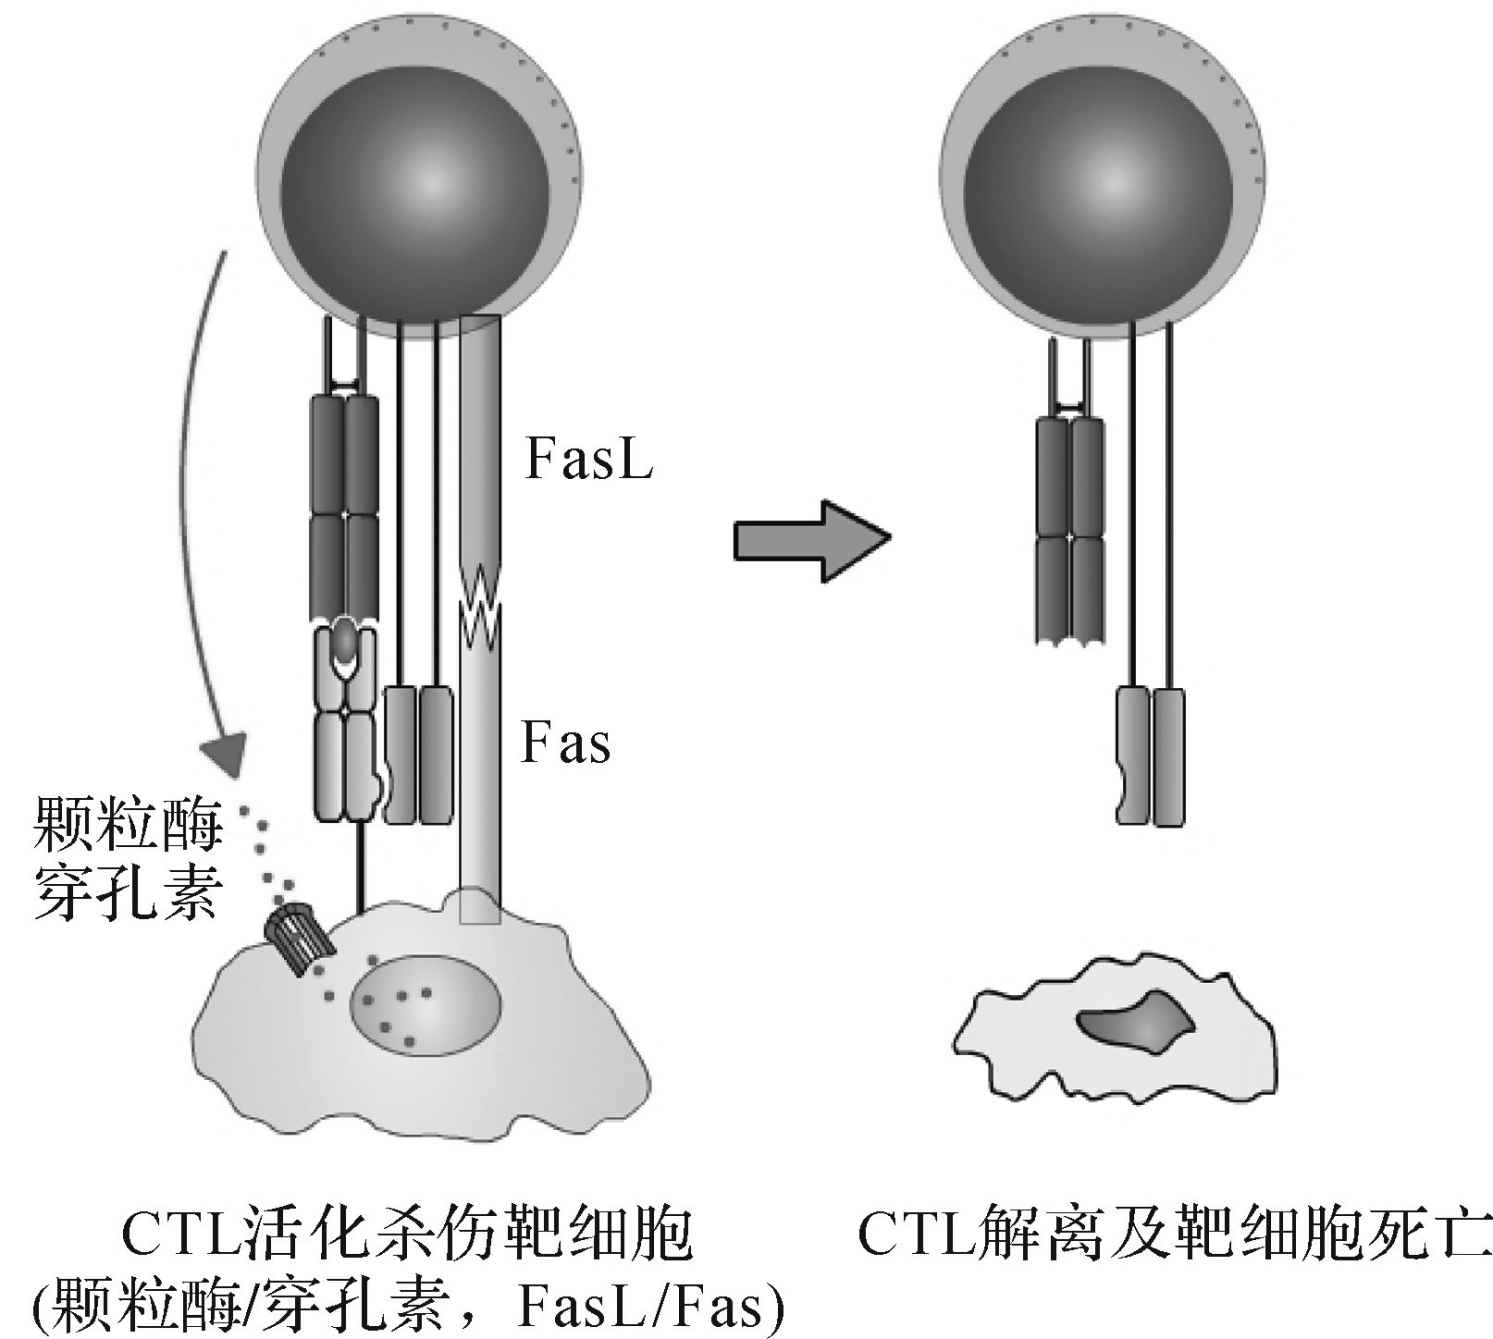
\includegraphics[scale=1.1]{./images/Image00021.jpg}
 \caption{CTL杀伤靶细胞示意图}
 \label{fig1-14}
  \end{figure} 

(四)造血与免疫细胞的发育

对人类细胞生成研究最为清楚的是免疫细胞,鉴定出多能造血干细胞(HSC),证明它能分化为不同类型的血细胞及免疫细胞。这项研究的推广,导致神经干细胞的发现,并证明它能分化为各类神经细胞和免疫细胞。现已有多种组织器官特异的干细胞被鉴定成功(图\ref{fig1-15})。

\begin{figure}[!htbp]
 \centering
 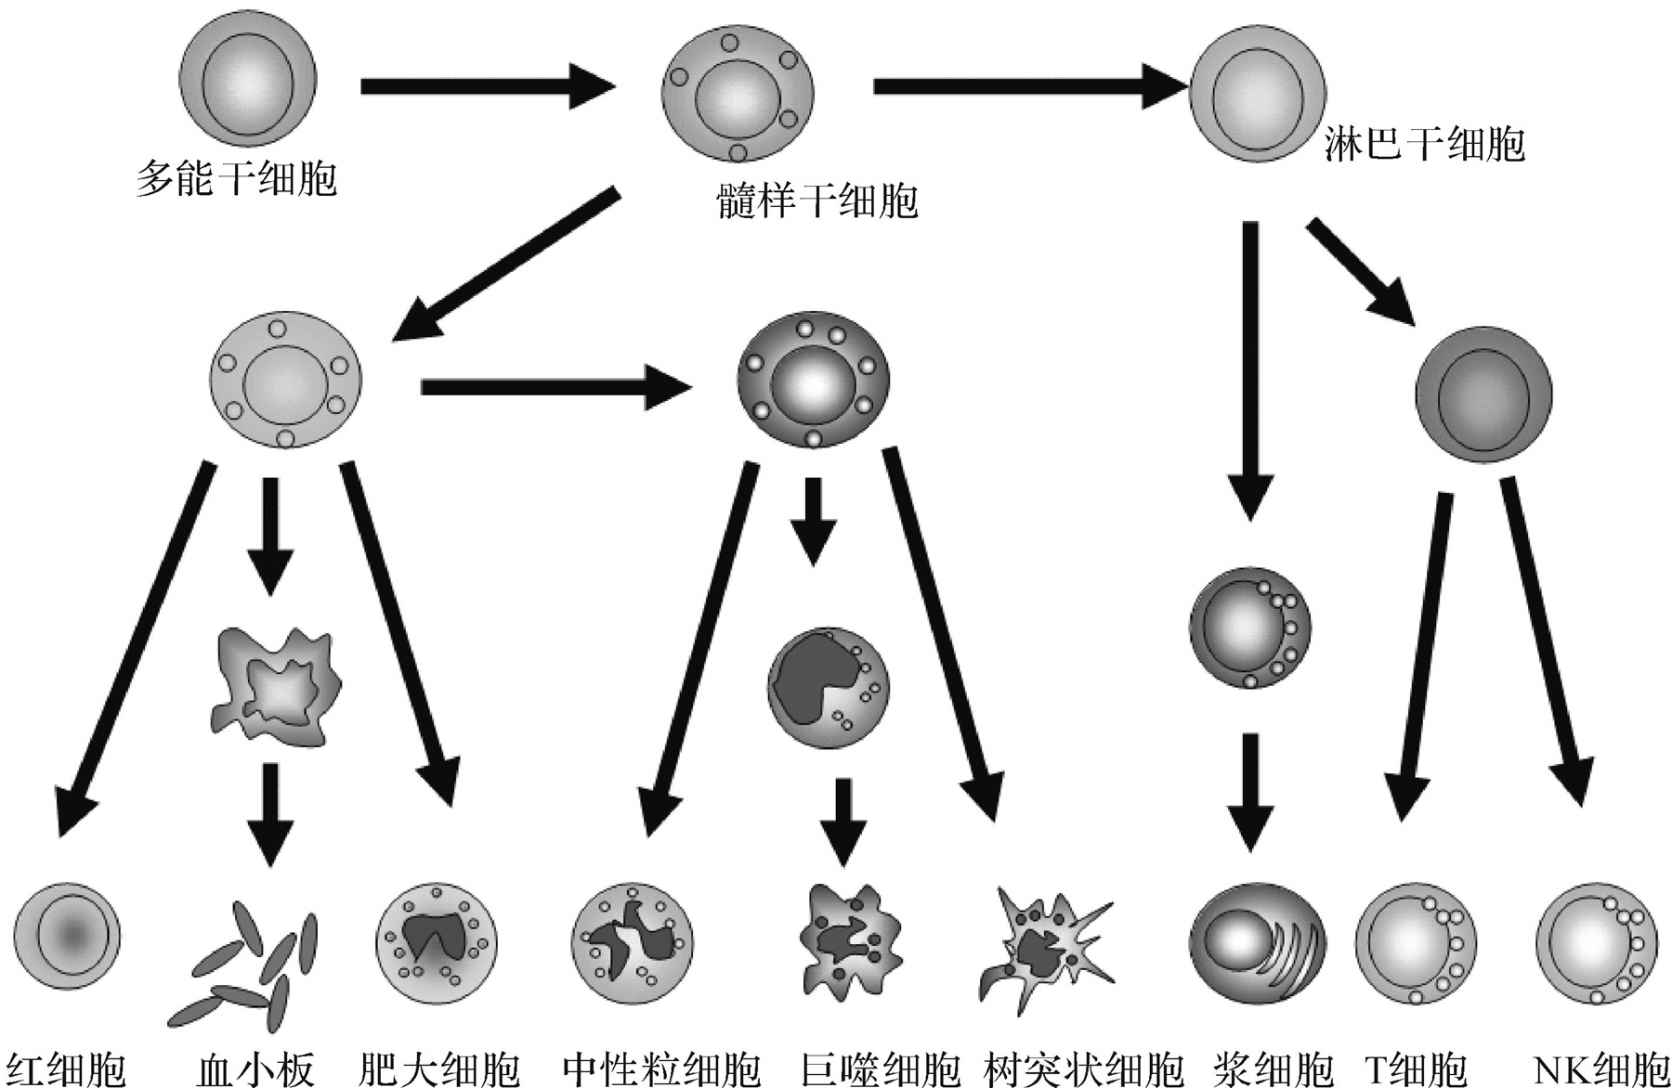
\includegraphics[width=.7\textwidth]{./images/Image00022.jpg}
 \caption{免疫细胞发育示意图}
 \label{fig1-15}
  \end{figure} 


\subsection{应用免疫学的发展}

应用基因工程开发免疫学制品,使之得以大规模廉价生产;新型细胞因子的发现及应用,使多种免疫细胞在体外扩增培养成功,用于临床;分子生物学技术的发展,使人源抗体问世;对免疫途径及效应识别的了解,提供了预防自身免疫病的新途径。免疫学应用研究已在更广阔、更高水平上得以开拓。

(一)DNA 疫苗

在鉴定出病原体引起免疫应答的蛋白抗原及其编码基因后,已发展起 DNA
疫苗,如乙型病毒性肝炎(HBV)DNA疫苗,在使用中效果显著。DNA
疫苗成本低、活性稳定、运输容易,甚至用基因转入食物细胞,如西红柿细胞,口服长成的西红柿即可,不须纯化,是为理想的方法。DNA
疫苗亦可用于治疗基因缺陷所致的免疫缺陷病,如转染腺苷脱氨酶(ADA)基因治疗因
ADA基因突变所致的联合免疫缺陷症,是当今基因治疗中效果最为显著的典型。尽管DNA
疫苗在使用上仍存在诸多技术问题,但这是今后发展方向。

(二)基因工程制备重组细胞因子

应用大肠杆菌、酵母及昆虫细胞等生产人类基因重组细胞因子已广泛应用于临床,并已发展成为高生物科技的新型药物工业。人重组红细胞生成素(EPO)及粒细胞集落刺激因子(G-CSF)等的临床使用,效果显著,经济效应巨大,更多的重组细胞因子正在临床试用中。

(三)免疫细胞治疗

造血干细胞及效应细胞毒性 T
细胞在适宜细胞因子存在的条件下,已能体外培养扩增,用于临床治疗。DC细胞的体外分化成熟,用以递呈抗原,使
T 细胞活化效果显著提高,已用于肿瘤治疗。

(四)完全人源抗体

抗体治疗已在抗感染、抗肿瘤、抗自身免疫病中广泛使用,但不同动物种属来源的抗体,在应用中有致过敏的危险,且多次使用会致失效。现已能用小鼠制备人的抗体,即将小鼠免疫球蛋白(Ig)基因全部或大部分敲除,转入人
Ig
基因,培育成的小鼠,在抗原刺激下,能产生完全人源的抗体,其效果提高,且因无小鼠成分不会被排斥。

(五)免疫生物治疗

DNA疫苗,基因工程抗体靶向治疗、基因工程细胞因子和其他肽类分子等均已开始在临床得到应用;细胞过继疗法已用于多种血液病及肿瘤的治疗。一般认为,肿瘤的免疫生物治疗有可能成为继化学疗法、手术疗法、放射疗法之后的又一重要疗法(图\ref{fig1-16})。

\begin{figure}[!htbp]
 \centering
 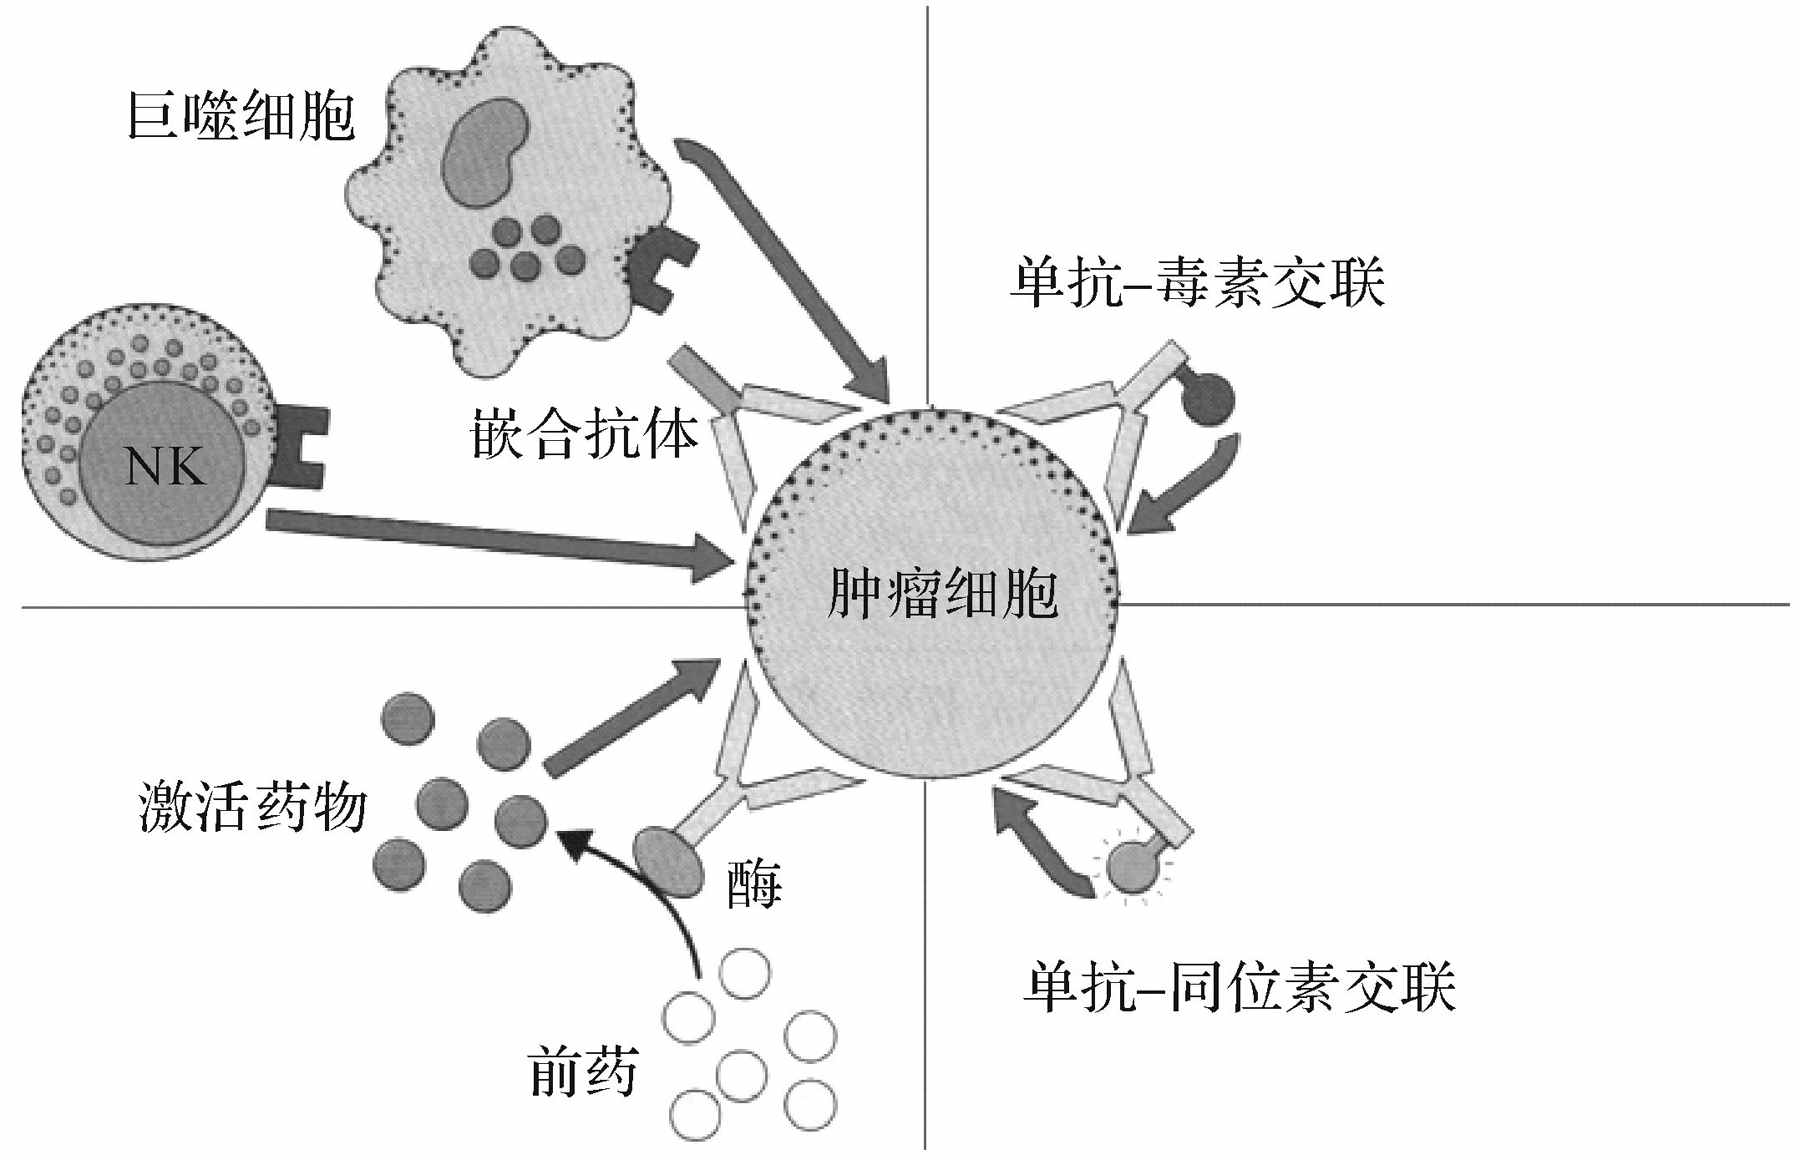
\includegraphics[scale=1.2]{./images/Image00023.jpg}
 \caption{免疫生物治疗示意图}
 \label{fig1-16}
  \end{figure} 

\section{免疫学在生命科学中的重要地位}


\subsection{免疫学促进了生命科学发展}

作为一门新兴的交叉学科,免疫学研究进展为生命科学的持续发展不断注入新的活力,尤其对阐明生命活动的本质提供了重要线索。

1.免疫应答涉及复杂的细胞间信息交通、细胞内信号转导和能量转换,阐明其本质,有助于深化对生命过程中诸多生物学现象基本特性的认识。

2.广义上,机体所有生理功能均受遗传控制,但迄今对其确切机制知之甚少。近20年来免疫遗传学(以MHC/HLA为主要研究目标)进展迅速,揭示了遗传控制机体免疫应答的机制,从而为在基因水平探讨机体生理功能展示了全新前景。

3.随着许多基本免疫生物学现象的本质不断被阐明(如MHC的结构和功能、免疫球蛋白基因表达的等位排斥、免疫球蛋白及其他免疫因子的分子生物学特征、细胞因子表达及其调控机制等),极大地拓宽了分子生物学的研究领域,并深化了对真核细胞基因结构和表达调控的认识。

4.日新月异并不断完善、改进的免疫学技术和试剂,为生命科学研究提供了有力手段。


\subsection{免疫学极大促进了生物技术及生物产业发展}

免疫学从其建立之日始,所取得的每一重要进展均对生物技术及产业起巨大推动作用,形成极富生命力的“基础研究-应用研究-高科技开发”发展模式。在免疫学建立之初,抗感染免疫研究进展有力推进了以疫苗研制为主的生物制品产业发展,并使人工主动免疫和被动免疫得以广泛应用。近30年来,现代免疫学在更深层次和更广范围内推动了生物高技术产业发展。目前,以细胞因子和单克隆抗体为主要产品的生物制药,已发展成具有巨大市场潜力的新兴产业。

纵观免疫学的发展史,以及免疫学及其分支学科引人注目的进展,免疫学当之无愧地与神经生物学、分子生物学并列为生命科学三大支柱学科之一。作为支持这一评价的佐证之一,现将整个20世纪获得诺贝尔医学生理学奖的免疫学家及其主要成就列成表(表\ref{tab1-3})。
 
\begin{longtable}{lllp{5cm}}
    \caption{20世纪获得诺贝尔医学生理学奖的免疫学家及其获奖成就}
    \label{tab1-3}\\
    \toprule
    年代&学者姓名&国家&获奖成就\\
    \midrule
    \endhead
    1901&Behring&德国&发现抗毒素,开创免疫血清疗法
\\
1905&Koch&德国&发现病原菌
\\
1908&Ehrlich&德国&提出抗体生成侧链学说和体液免疫学说
\\
1908&Metchnikoff&俄国&发现细胞吞噬作用,提出细胞免疫学说
\\
1912&Carrel&法国&器官移植
\\
1913&Richet&法国&发现过敏现象
\\
1919&Bordet&比利时&发现补体
\\
1930&Lands teiner&奥地利&发现人红细胞血型
\\
1951&Theler&南非&发明黄热病疫苗
\\
1957&Bovet&意大利&抗组胺药治疗超敏反应
\\
1960&Burnet&澳大利亚&提出抗体生成的克隆选择学说
\\
1960&Medawar&英国&发现获得性移植免疫耐受性
\\
1972&Edelman&美国&阐明抗体的化学结构
\\
1972&Porter&英国&阐明抗体的化学结构
\\
1977&Yalow&美国&创立放射免疫测定法
\\
1980&Daus set&法国&发现人白细胞抗原
\\
1980&Snell&美国&发现小鼠 H2系统
\\
1980&Benacerraf&美国&发现免疫应答的遗传控制
\\
1984&Jerne&丹麦&提出免疫网络学说
\\
1984&Kohler&德国&杂交瘤技术制备单克隆抗体
\\
1984&Misls tein&英国&单克隆抗体技术及免疫球蛋白基因表达的遗传控制
\\
1987&Tonegawa&日本&抗体多样性的遗传基础
\\
1990&Marray&美国&第一例肾移植成功
\\
1990&Thomas&美国&第一例骨髓移植成功
\\
1996&Doherty和Zinkernagel&美国&提出 MHC限制性,即 T细胞的双识别模式\\
    \bottomrule
    \end{longtable}







\subsection{现代生物学进展促进了免疫学发展}

现代生命科学的特点之一是,多学科间表现出极为明显的相辅相成和互动性。现代生物学在过去数十年间取得的巨大进展,也有力促进了免疫学发展。

1.现代生物学进展拓宽并深化了免疫学理论和应用研究,依托现代细胞生物学、分子生物学和分子遗传学等学科的研究进展,使得有可能在分子和基因水平阐明基本免疫学现象的本质。

2.现代生物学技术------推动免疫学发展的催化剂。

(1)基因操作与分析技术:基因打靶和各类反应技术可用于分析特定免疫分子或细胞内信息分子的生物学功能;大规模DNA测序、新型基因分析技术(如限制性片段长度多态性、微卫星、单核苷酸多态性分析等)和DNA芯片等技术被建立,并不断提高其检测灵敏度和分辨率,从而有可能进行快速、高通量的基因分析;多聚酶链式反应及其层出不穷的衍生技术,更为分子免疫学研究提供了有效手段。

(2)蛋白分析技术:借助基因工程技术,使得有可能按人们的意愿获得各种免疫分子或其融合蛋白,并被广泛应用于免疫学研究领域;有赖于蛋白纯化技术的不断完善,可获得稳定的蛋白结晶体,用于分析免疫分子的三维结构;噬菌体肽库、酵母双杂交、计算机分子模拟技术等,可用于分析抗原表位和/或免疫分子间的相互作用;氨基酸多肽合成技术可用于分析多肽分子间细微的结构差异及其生物学功能的改变,并指导新型疫苗和药物设计;二维电泳可用于分析复杂的蛋白谱,并发现新的免疫功能分子;微量传感器(microsensor)可用于检测蛋白质、酶、胞内信息分子活性,并对抗体-抗原、受体-配体的结合及其亲和力进行分析。

(3)细胞与组织学技术:杂交瘤技术的建立为制备单克隆抗体奠定了基础;造血/胚胎干细胞培养与定向分化技术的完善,使得有可能深入研究免疫细胞的分化、发育及其调控;细胞分离技术(流式细胞分选、激光显微切割仪、免疫磁性微球等)和显微观察、分析技术(流式细胞术、激光共聚焦显微镜、隧道扫描显微镜、计算机成像与图像分析技术)为分析特定细胞群或单一细胞的生物学特征提供了工具。

\section{教材基本轮廓}

本教材主要适合于生物技术与生物工程专业学生使用,有关免疫病理等内容不在其中。共三部分组成,分别为免疫基础、免疫应答、免疫学应用,分为十二章,包括如下内容:

1.免疫基础:包括免疫系统、抗原、免疫球蛋白、补体、细胞因子、主要组织相容性系统、白细胞分化抗原。

2.免疫应答:涉及抗原递呈细胞、抗原的递呈与加工、T细胞介导的细胞免疫应答、B细胞介导的体液免疫应答等。

3.免疫学应用:涉及免疫检测、免疫治疗、免疫预防和免疫制剂等。

全书以“矛”------抗原与“盾”------免疫系统两方面为主线展开,着重点是免疫系统的构成,从免疫器官、免疫细胞(种类、功能及免疫细胞膜分子)、免疫分子(抗体、补体、细胞因子,主要由免疫细胞产生)为主线讲述,各章节间均有内在必然联系,具有一定的系统性和完整性,各章节的内容和插图有某些重复与交叉。图示为本教材所涉及内容的基本轮廓和编排思路,也反映了各章节间的联系。
\begin{center}
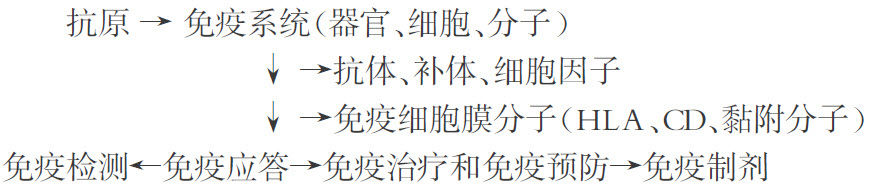
\includegraphics[width=0.7\textwidth]{./images/Image00024.jpg}
\end{center}
{\textbf 【课外拓展】}

1.免疫学与别的学科如临床医学、检验学、食品科学等有何关系?

2.阐述免疫制剂与生物产业的关系。

{\textbf 【课程实验与研究】}

1.在2009年1月,中科院生物物理所感染免疫中心唐宏研究员和傅阳心教授在《免疫学趋势》(Trends
in Immunology)杂志上以《Do adaptive immune cells suppress or activate
innate
immunity》为题,系统阐述了他们近来提出的“天然免疫反应需要T细胞参与”的新理论。如果你是课题组成员,如何来证明这一新理论?

2.免疫系统如何识别病毒入侵从而迅速产生干扰素、有效地触发天然抗病毒免疫防御功能进而清除病毒感染,是生命科学与医学研究中的重大科学问题。你能查阅资料,撰写一篇综述性文章吗?

3.2008年生物产业发展情况调查数据已经发布,如果请你了解一下周围人群对免疫制品的熟悉程度和需求,你能设计一张调查问卷吗?

4.你能针对你所掌握的情况,列出医学等领域与免疫学有关的急需解决的问题吗?你能设想二十年后,免疫学会给我们健康带来哪些变化?请你写篇科幻小论文,展示免疫学的前景。

{\textbf 【课程研讨】}

1.生锈的铁钉深度刺进体内,可能会得什么病?机体免疫系统会发生如何反应?为何?

2.同样的外界条件,有人生病了,有人却健康,为何?

3.请以某一科学家科学探索和成长经历为例,阐述我们的大学学习该如何为将来的成才打下扎实的基础。

4.免疫对机体的作用一直是正面的吗?请从正反两方面加以阐述免疫的作用。

5.从你自身或周围人群的需要出发,请列举免疫学研究热点问题。假设你是免疫学家,请设计研究方案与技术路线。

{\textbf 【课后思考】}

1.何谓免疫?举例说明免疫的基本特性、基本功能及功能异常的表现。

2.简述固有性免疫(非特异性免疫)和适应性免疫(特异性免疫)的概念和特征。

{\textbf 【课外阅读】}
\begin{center}
{\Large 我国免疫学研究概况}
\end{center}
\begin{center}
{\large\textbf 一、 我国免疫学研究的历史}
\end{center}

过去国外学者将免疫学的开创归功于英国乡村医生 Edward Jenner
(1749---1823)于1798年给一名男孩接种牛痘(见于国外绝大多数免疫学教科书),而我们中国免疫学者往往自豪地讲免疫防治的经验始于中国唐宋年间的民间人痘接种(见于国内免疫学教科书),其实,我们中国学者应该更自豪地讲,免疫防治的概念最早萌芽于我国东晋时代医学家葛洪(281---341),他在公元303年左右所著的《肘后备急方》中记载了有关医治“癫疯狗病”的方法(仍杀所咬犬,取脑敷上,后不复发),即描述了应用病犬的脑髓敷伤口以防治(可能的)狂犬病,所以,世界免疫学的历史始于中国,而且是距今1700年前。

我国近代免疫学的研究工作起步并不太晚,涌现出很多优秀免疫学家,而且也取得过多方面的免疫学实际应用研究成果。最早的免疫学研究可以追溯到上世纪
30 年代,刘思职教授(1904---1983) 于1930年至 1942
年在北平协和医学院工作期间(1942年之后执教于北京大学医学院),与世界著名的我国生物化学学科的奠基人吴宪教授(1893---1959)
合作,开创了我国免疫化学的研究,创造性地用化学定量方法研究抗原抗体的沉淀反应,纯化了抗体,在国外英文学术杂志发表了两篇有关免疫沉淀反应定量研究的论文;也在协和医院工作的谢少文教授(1903---1995)开创性地建立了立克次体的体外鸡胚培养扩增体系、建立了立克次体病的免疫学检测方法、发展了灭活立克次体疫苗的制备体系;同时代在上海工作的两名著名免疫学家对于我国免疫学研究的开展也做出了重要贡献,上海第二医学院余贺教授(1903---1988)于1933年提出了过敏介导的风湿热发病学说,上海医学院林飞卿教授(1904---1998)研究了细菌感染的免疫学应答反应。这四位前辈大家的工作奠定了我国免疫学研究的早期基础。前中国医学科学院院长顾方舟教授
50 年代从前苏联留学回国后,于 1960 年、 1962
年先后研制成功脊髓灰质炎减毒活疫苗以及“脊灰”减毒糖丸活疫苗,为我国消灭“脊灰”做出很大贡献。侯云德院士
1962
年从前苏联留学回国后在中国医学科学院和中国预防医学科学院病毒学研究所从事病毒研究工作,于
70 年代开始了干扰素研究,并于 80
年代初发现和制备了重组α1β型干扰素,并于1992年获得新药证书,完成了第一个由我国学者自己发现的、具有自主产权的免疫产品。1960年从前苏联医学科学院风湿性疾病研究所进修回国的张乃峥教授在全国最先建立了风湿性疾病门诊,并于1979
年在协和医院首次成立了“风湿病科”,标志着我国科研、教学与患者临床治疗一体化的临床免疫学及风湿病学科的开始。70年代在实验设备非常简陋的条件下,中国医科院肿瘤研究所张友会教授创建了有自己特色的巨噬细胞研究体系并得到国际同行的高度评价。该所的孙宗堂教授建立了火箭电泳法检测甲胎蛋白,应用于早期肝癌的检测;上海医学院(现复旦大学上海医学院)汤钊猷教授将通过甲胎蛋白筛查出来的早期肝癌病人进行及时手术、提出了“小肝癌”防治的概念,成为我国具有国际学术影响力的标志性医学成果。中国预防医学科学院病毒学研究所曾毅院士在
EBV与鼻咽癌发生发展的关系以及肿瘤病毒的抗体反应基础研究与临床应用方面(广西鼻咽癌高发现场的流行病调查、早期诊断与干预)做出了开创性工作。杨贵贞教授留苏归国后,在神经内分泌免疫调节以及中药免疫研究方面取得了一系列成果。

“文革”结束后,我国的老一辈免疫学家们对于尽快恢复、提高我国的免疫学研究做出了积极的努力,谢少文教授和杨贵贞教授举办了多次免疫学新技术新理论学习班,培养了一批后来在我国各大研究机构和大学里对于推动我国免疫学研究发挥了很大作用的免疫学骨干力量。第二军医大学叶天星教授(1915---1999)于1979年3月编写出版了我国第一本全面系统介绍免疫学现代理论与方法的免疫学教科书《免疫学理论与实践》。天津医科大学郑武飞教授于1989年5
月编写出版了我国第一本医学院校本科生《医学免疫学》教材(人民卫生出版社),北京医科大学龙振州教授于1992年召开了全国免疫学教学研讨会、并于1995年主编了全国医科院校《医学免疫学》统编教材。在
80---90
年代,很多杰出的免疫学家包括汪美先教授(1914---1993)、赵修竹教授(1920---2003)、朱锡华教授(1922---2008)、卢景良教授(1930---2000)、王亚辉教授(1929---1999)、叶敏教授(1930---2005)、钱振超教授、崔正言教授、何球藻教授、马宝骊教授、孔宪涛教授、葛锡锐教授、章谷生教授、郑振群教授、许贤豪教授、宗庭益教授等除了在各自的研究领域做出了重要贡献外,还积极创办了中国免疫学会多个专业分会/委员会以及地方免疫学会,创办了
7
份隶属于中国免疫学会的学术期刊,编写或参与编写了不同类型的免疫学教材和免疫学专著,对于免疫学现代理论与技术在我国的普及与教育做出了重要贡献。与此同时,一批杰出中青年学者受国家公派留学欧美、澳大利亚、日本等,巴德年院士
1982 年在日本北海道大学医学癌症研究所获博士学位,回国后于 1986
年在国内开展了第一个细胞免疫治疗临床试验。陈慰峰院士 1982
年在澳大利亚墨尔本大学获博士学位,回国后建立了胸腺
T细胞分化发育实验室,为我国基础免疫学研究的开展起了重要的带头作用。沈倍奋院士、闻玉梅院士于80年代初留学英国,回国后分别在
CD 抗原的单抗与白血病免疫分型、HBV
免疫学与乙肝疫苗研制等方面做出了开创性工作。董志伟教授从美国留学回来后推动了我国抗肿瘤单抗制备与应用工作。同期从国外留学归来的医科院血液学研究所陈璋教授、军事医学科学院白炎研究员、武汉生物制品研究所史良如研究员、上海市中心血站赵桐茂研究员、
第四军医大学崔运昌教授均在单克隆抗体领域做出了杰出贡献,其中,我国第一个获得上市销售的单抗产品“抗肾移植OKT\textsubscript{3}
---注射用鼠源性抗人T淋巴细胞
CD3抗原单抗”由武汉生物制品研究所研制成功。此外,分别从美国、德国、澳大利亚留学归来的周光炎教授、龚非力教授、金伯泉教授在免疫遗传与免疫调节、HLA
与移植耐受、CD免疫分子与单抗等领域做出了杰出工作,并且各自主编了免疫学的教科书,推动了国内免疫学教学工作,培养了很多免疫学新生力量。随后,很多中青年免疫学工作者成长起来,成为当今我国免疫学研究的中坚力量,并在推动我国免疫学研究走向世界的过程中发挥了积极作用。

在中国免疫学走向世界的历程中,值得我们纪念的是中国医学科学院的吴安然教授(1922---2005),吴教授是1986年向国家科委提议成立“中国免疫学会筹委会”的主要专家(于1984年8月经中国科协国际部批准成立“国际免疫学会联合会中国委员会”,于1988年10月获得国家科委批准正式成立中国免疫学会),并作为我国首任国际免疫学会联盟(IUIS)执委,推动了中国免疫学会与
IUIS的交流合作。

\begin{center}
{\large 二、我国免疫学研究的整体现状及其与国际同领域的比较}
\end{center}

我国早期的免疫学工作者多在医科院校的微生物教研室、病理教研室或者肿瘤学实验室、医院检验科,直到20世纪80年代末90年代初,免疫学教研室或者实验室才得以独立,90年代末本世纪初才成立免疫学研究所,直到近年来综合性大学和国立科研机构才成立免疫学研究所/中心。由于学科发展的自身特点以及受到国家资助较少等历史原因,使得过去我国免疫学研究(从学科整体的角度看)的基础相当薄弱,受限于科研条件,很多优秀免疫学家只能以教学为主或者侧重于(已有的)
免疫学技术的建立、改良与应用,或者集中于血清学和免疫学诊断、免疫预防(疫苗制备、计划免疫等),较少涉及关键性免疫学基本科学问题的理论研究,很少创建具有开拓性的免疫学技术,也很少具有自主知识产权的免疫制品过渡于临床应用或者经过
SFDA
正式批准上市的免疫产品。尽管我国免疫学研究起步较晚,但免疫学领域的成果在我国生物医学等方面的应用尤其广泛并产生了巨大的社会和经济效益,在我国卫生防疫事业尤其是人口健康和生命科学领域的发展过程中发挥了十分重要的作用。如多种感染性病原微生物疫苗的研制和应用大大提高了我国人民的健康水平,乙肝疫苗的研制和应用极大地降低了乙肝的发病率,也有效地预防了肝癌的发生。

英国和法国是免疫学研究的传统强国,在历史上取得过很多对人类具有重大贡献的免疫学成果,但近二十年来,由于这些国家在科研总体经费,尤其是基础研究经费投入的不足,其免疫学的发展速度被美国赶超,尽管最近这些国家也意识到这方面的问题并开始重新重视,但其发展势头明显不如美国,甚至有被日本赶超的趋势。由于免疫学涉及的领域和学科非常多,其投入的经费、产出的论文等难以精确统计,只能以局部的数据作为简单的比较。美国在免疫学领域投入非常大,如美国国立卫生研究院(NIH)的基金中,约15
\%用于免疫学研究,当然,其产出也是十分的惊人,在高级别免疫学杂志发表的论文中,在美国本土完成的工作占有很大的比例,其免疫学研究处于国际领先地位。此外,加拿大、澳大利亚等国在免疫学领域内做出了不少高水平的研究,印度在生殖免疫学及疫苗研制上也有其独特的成就。

利用 ISI Essential Science
Indicators数据库分析,对世界主要国家免疫学领域的科技论文数量及其总被引用次数分别进行统计显示,免疫学研究领域科技论文产出、被引用次数世界排名前5的国家均为美国、英国、日本、德国、法国,这5个国家发表的论文占免疫学领域研究论文总数78.45\%。1998年至2008年中国免疫学研究科技论文产出2000多篇,占全球免疫学研究论文总数的1.87\%,论文数排名第13位,被引用次数排名第21位。这些统计数字也表明,经济实力和科技水平高的国家,包括美国、英国、日本、德国、法国等其在免疫学领域的影响也特别大,处于免疫学研究的第一方阵,其中,美国作为一个科技大国,其免疫学研究也遥遥领先于其他国家。意大利、加拿大、荷兰、澳大利亚等国的免疫学研究处于第二方阵,我国和西班牙、韩国等处于第三方阵,领先于印度和俄罗斯。我国在免疫学研究方面发表的论文数尽管处于世界第13位,但其引用次数排名仅为第21位,从一个侧面反映出我国创新性、源头性的免疫学研究工作不多,缺乏具有中国特色的、具有突破性的理论研究成果,因此,中国免疫学研究的创新能力实际上应处于世界第20位左右。

免疫学研究领域科技论文产出世界排名前20的机构中,70
\%机构的国别是美国,其他国家的机构主要有法国巴斯德研究所、瑞典卡罗林斯卡医学院、日本东京大学和大阪大学、英国伦敦大学等。众所周知,这些机构均是创新性科技成果的发源地,也是高水平医学人才的摇篮。我国尚无这样高水平的研究机构,亟待我国相关部门的重视。从这些统计数据里也可以看出,对大多数国家而言,免疫学的发展水平与一个国家的科技经济水平呈正相关。我国的经济和科技事业在近年来取得了长足的进步,但免疫学的发展相对滞后,这与中国的经济实力不相称,也与科技事业的整体进步不相适应,因此,除了我国免疫学工作者需要加倍努力外,还需要国家在免疫学研究与应用方面加大投入,以促进其快速发展。

\begin{center}
{\large 三、我国免疫学研究的近期进展}
\end{center}

从20世纪90年代中后期开始,我国免疫学家逐步在国际免疫学杂志发表在本土完成的免疫学研究工作,论文的数量和质量不断提升,研究内容几乎涉及基础与临床免疫学的各个领域:

我国免疫学家在细胞与分子免疫学领域做了很多创新性工作。例如,北京大学医学部免疫学系陈慰峰院士实验室在T细胞分化发育以及近年来在新型肿瘤抗原的鉴定与功能研究方面取得了系列进展,去年在
PNAS发表论文,阐明了一个CD4SP胸腺细胞个体发育上以及功能上相关的成熟过程的机制,即髓质中CD4SP
细胞的发育可能严格依赖于一种功能上完整的髓质上皮细胞小室,Relb和Aire突变会引起SP3向SP4转变过程中的严重阻隔。同系的马大龙教授实验室自主克隆了多个编码细胞因子和凋亡相关分子的人类功能基因,其中
2个新分子即趋化素样因子1(CKLF1)和程序化细胞死亡分子5(PDCD5,过去命名为
TFAR19)
受到国际同行的关注。中国科技大学免疫学研究所田志刚教授实验室与山东大学免疫药理研究所合作在NK/NKT细胞的基础免疫学与肝脏免疫学领域开展了系列研究,尤其在NK/NKT细胞与肝炎发病机制研究方面具有国际影响,近期发现了NK细胞和Kupffer
细胞通过NKG2D/Rae1识别加重 NK细胞介导的肝炎,在建立 TLR3
信号诱导的小肠黏膜损伤模型的基础上发现NKG-D识别介导TLR3信号诱导的小肠黏膜损伤,先后在
PNAS、Hepatology等杂志发表论文。中国医学科学院基础所何维教授实验室在γδT细胞的免疫学特性以及通过
CDR3delta 区域识别靶细胞的研究很有创新性,论文发表在 Cancer
Res和JBC。除了近来集中研究
Th17以外,中山大学医学院吴长有教授实验在JI、Blood杂志报道了结核杆菌(MTB)感染机体导致慢性感染之后为何机体不能有效地清除MTB的机制,发现与结核患者体内调节性T细胞增加、调节性T细胞反过来抑制CD\textsuperscript{+}
\textsubscript{4} T细胞和人记忆性γδT细胞在结核杆菌抗原 ESAT-6
刺激下产生IFN-γ密切相关;同院的郑利民教授实验室在Blood、Cancer Res
报道了他们对于肿瘤微环境中巨噬细胞功能低下机制和Th17与肿瘤的关系。苏州大学免疫学研究所的张学光教授实验室对于淋巴细胞的共刺激分子活化信号网络开展了多年研究制备了抗共刺激分子的系列单抗,其中有的活化型单抗和中和性单抗具有很大的临床应用价值。中国医学科学院基础所郑德先教授实验室除了研究淋巴细胞受体及相关基因的表达调控、信号传递及其在机体免疫调节和自身免疫性疾病中的作用外,还制备了抗TRAIL受体
DR5 的单克隆抗体(AD5-10),在 Cancer
Res、JBC等杂志发表论文证明其可以触发凋亡信号通路、发挥抗肿瘤作用。

免疫识别与免疫应答的分子机制是免疫学研究的重要前沿领域,我国学者的数项工作在国际同行中颇有影响。中科院上海生命科学院裴刚院士实验室在
beta-arrestin与 TLR 触发炎症信号转导调控和CD\textsuperscript{+}
\textsubscript{4} T细胞存活机制的作用的研究结果,两次发表在Nature
Immunology。该院孙兵教授实验室在
Th1、Th2细胞分化的分子机制、炎症性因子的分子调控机制的研究结果发表在
Nature
Immunology。北京大学/武汉大学生命科学院舒红兵教授实验室发现了VISA蛋白在病毒触发干扰素产生中的重要作用(这个蛋白分子也被国际同行称为MAVS,IPS-1,Cardif),论文发表在
Mol Cell
并受到广泛引用。第二军医大学免疫学研究所暨医学免疫学国家重点实验室曹雪涛等与浙江大学免疫学研究所合作,提出了成熟树突状细胞在基质微环境中再分化并形成新型调节性树突状细胞的观点,还发现了多种免疫分子和信号分子(如
SHP-1、SHP-2、PECAM21等)参与了TLR及RIG-I免疫识别与炎症性细胞因子、干扰素产生的调控,先后在Nature
Immunology发表两篇论文、在 Immunity发表一篇论文。

免疫调节与免疫耐受的机制及其与免疫性疾病的关系是当今基础与临床免疫学中的热门研究领域。北京大学医学部免疫学系高晓明教授实验室在国内较早开展了调节性T细胞的研究,近来发现多种抗多糖特异性抗体参与调节性T细胞的作用和自身免疫性疾病的发病过程。中科院上海健康研究所臧敬五教授实验室发现了IFN-γ和OPN在调节性T细胞的形成与作用机制中的重要作用,论文发表在JCI和
PNAS。中科院动物所赵勇教授实验室在调节性T细胞与移植免疫耐受的研究有新的观点,在Trends
Immunol
上发表综述系统介绍了该领域的研究工作。军事医学科学院黎燕教授/沈倍奋院士实验室研究了抗
CD3抗体诱导免疫耐受、逆转NOD小鼠糖尿病发病的机制,证实 NKT细胞及
TGF-β在其中发挥重要作用,发现将自身抗原与
IgG分子融合诱导免疫耐受的机制主要与有效诱导调节性T细胞的产生,逆转体内
T细胞极化失衡有关。

国内有多家实验室在重大疾病发生发展的免疫学机制与免疫治疗领域开展了卓有成效的研究工作。HBV感染与乙肝疫苗的研究是我国学者的特色领域之一,第三军医大学免疫学研究所吴玉章教授实验室除了鉴定和研究了多种抗原表位并建立了表位数据库外,通过基于表位的免疫原设计(
EBVD)策略、研发了新型乙型肝炎疫苗,目前正在开展Ⅱ期临床试验。北京302医院王福生教授实验室在Gastroenterology、JI等杂志发表系列论文,分析了慢性乙肝以及肝癌患者调节性T细胞的变化和
PD-1在免疫功能低下中的作用,发现肝癌病人体内增加的调节性T细胞可导致CD\textsubscript{8}
T淋巴细胞功能损伤和病人的存活期缩短,其结果有助于人们深入认识慢性乙肝发展为肝癌并导致免疫功能低下的机制。复旦大学医学院熊思东教授实验室近来发现活化淋巴细胞的DNA具有一定的诱导自身免疫性疾病的作用,目前正在研究其作用机制,有望为自身免疫性疾病的发生发展机制提出新的解释。四川大学华西医学院生物治疗国家重点实验室魏于全教授实验室提出了将生物进化中的异种同源基因与异种免疫排斥反应及自身免疫反应相结合用于探讨肿瘤治疗、可以克服自身抗原的耐受性的新观点,为肿瘤疫苗及抗肿瘤血管治疗研究提供了新思路,在Nature
Medicine上发表论文后引起了国际同行的极大关注。第四军医大学免疫学教研室杨安钢教授实验室在Hepatology、Cancer
Res等发表了系列论文,系统报道了重组免疫促凋亡分子的内化及转运作用机制以及抗肿瘤作用,研制出的单抗介导的肝脏靶向性的基因干预体系具有潜在的免疫治疗应用价值;第四军医大学细胞工程中心陈志南院士实验室长期研究HAb18G/CD\textsubscript{147}
在肿瘤免疫治疗中应用及其作用机制,放射性同位素标记的HAb18G成为我国SFDA正式批准上市的第一个肝癌治疗用单抗药物。

还有一些实验室在某些免疫学前沿领域开展了探索性研究,例如,军事医学科学院沈倍奋院士实验室近年来在受体/配体相互结合与动态作用的分子模建、抗体的结构分析的平台技术体系等有了重要进展;中山大学生命科学院徐安龙教授实验室以文昌鱼为模型研究了免疫进化机制,提出了新的免疫发生的机制;华南理工大学生命科学院王小宁教授实验室几乎与国际同行同步提出了免疫受体编辑的观点并开展了实验研究;中科院微生物研究所高福教授实验室在免疫分子和病原体组分的结构生物学前沿领域也开展了令国际同行关注的工作。

在我国本土免疫学研究取得长足进步的过程中,我们不得不感谢那些虽身在海外但一直关心和扶持国内免疫学发展的一大批杰出华裔免疫学家,他们为缩短中国免疫学研究与国际先进水平的差距起到了桥梁作用,为提高华人在国际免疫学领域的学术影响力起了重要作用。例如,MDAnderson癌症中心的免疫学系主任、pDC的发现者刘永军教授;共刺激因子的国际权威、霍普金斯大学医学院皮肤病免疫学系主任陈列平教授;免疫调节与免疫病理专家、芝加哥大学傅阳心教授;免疫识别与干扰素信号转导专家、加州大学洛杉矶分校程根宏教授;细胞因子与Th17专家、MD
Anderson癌症中心的免疫学系董晨教授;TNF家族分子的功能与信号转导专家、滨州大学陈有海教授;淋巴细胞分化发育专家、奥克哈姆医学中心孙晓红教授;肿瘤免疫学专家、贝勒医学院王荣福教授;分子免疫学与肿瘤免疫学专家、密执安大学肿瘤免疫中心主任刘阳教授;细胞因子信号转导专家、克利夫兰医学研究中心李晓霞教授;树突状细胞专家、澳大利亚WEHI研究所吴力教授;T细胞与免疫调节专家、加拿大多伦多大学张丽教授;HIV与CTL专家、英国牛津大学徐小宁教授;移植免疫学专家、日本国立儿童健康研究所李晓康教授等等。他们多次回国举办免疫学前沿进展报告会,或者合作成立联合实验室、研究组,为我国免疫学近年来的进步起了推动作用。例如,刘永军、陈列平、傅阳心、程根宏等“海外团队”与中科院生物物理研究所唐宏教授等一起成立了“感染与免疫”研究中心,将国际先进的技术与理念与国内实验研究相结合,在免疫调节机制与病毒感染的免疫应答机制研究方面取得了显著进展,已经在Nature
Medicine、
PNAS等发表论文,产生了很好的合作效果。此外,我国香港地区与台湾地区的免疫学研究也取得了进展,并且与内地免疫学界的交流与合作正日益加强。

\begin{center}
{\large 四、我国免疫学研究的未来}
\end{center}

我国免疫学研究近年来进步很快、生长点很多、技术平台已经建立、研究队伍已经基本形成、研究方向逐步明确,研究目标进一步凝练,有理由相信我国的免疫学研究将在未来的
10 年或者 20 年内实现跨越式发展,达到国际先进水平。以2008
年我国学者在国际免疫学研究领域的顶尖杂志Nature
Immunology连续发表5篇论文(分别由中科院上海生命科学院孙兵实验室、刘晓龙实验室和葛宝学实验室、军事医学科学院张学敏实验室、第二军医大学曹雪涛实验室发表)和1篇述评(第二军医大学曹雪涛)为例,可以看出我国免疫学基础理论研究的强劲势头;
从2008年11月在西安召开的第六届全国免疫学大会的1000人参会规模、大会和分会场学术报告的水平创历史新高以及中国免疫学会及各分会的学术纽带作用越来越大来看,我国免疫学研究的人才基础与创新性学术交流环境、氛围已经成熟;从结题的国家自然科学基金免疫学重大项目以及刚刚获得资助的国家自然科学基金免疫学重大项目和973计划、863项目、国家创新药物/传染性疾病两个重大专项的资助以及国家“211”“985”工程对于某些免疫学重点实验室的支持来看,我国免疫学研究的国家资助体系正在显著加强,为免疫学实验室平台体系的建设与课题研究提供了保障;从近年来大量海外免疫学家回归创办实验室或者与国内合作者共同创办免疫学研究中心或者共同申请基金项目以及国际间免疫学学术会议的广泛交流,为我国免疫学研究的国际前沿化提供了技术与智力支撑,特别是一流海外免疫学家例如
T细胞免疫学专家、美国新泽西州医科大学时玉坊教授和分子免疫学家、美国Scripps研究所韩家淮教授近期全职回国(分别回到中科院上海健康研究所和厦门大学),为我国免疫学界增加了新的重要力量;这些软硬件条件的改善与提高为我国免疫学研究的腾飞奠定了雄厚的基础。

但是,在充满希望和信心的同时,我们应该清醒地认识到与免疫学学科本身在整个医学与生命科学中重要性相比,我国免疫学研究在国家科技创新体系甚至医学与生命科学领域中的地位尚不够凸显,我们与发达国家免疫学研究水平尚存在较大的差距和不足,例如,虽然研究内容比较广泛,但是山多峰少、亮点不多,尚缺乏受到或者有可能将受到国际同行认可的免疫学研究的独特性技术体系、突破性学术观点或者原创性免疫学学术思想,尚缺乏特色系统理论的积累以及能够冲击传统免疫学观点的挑战性工作,几乎没有开创性的能够让国际同行追踪的研究方向与新研究领域的工作,也几乎没有我国学者首先发现而令国际同行追随的“明星免疫分子”或者“明星免疫细胞”,尚没有在国际免疫学领域受到国际同行公认的领军型的一流免疫学家(不能与美国国际一流免疫学家相比,即使与日本相比,我国本土还没有像发现调节性T细胞的
Shimon Sakaguchi(东京大学)、TLR/RIG-I研究权威Shizuo Akria
(大阪大学)、率先克隆IRF和IL-2等细胞因子信号转导权威Tada Taniguchi
(东京大学)、IL-6/gp130的发现者Tadamitsu Kishimoto
(大阪大学)、AID的发现者与B细胞抗体产生分子机制研究的权威 Tasuku Honjo
(京都大学)等有国际影响力的免疫学家),还没有任何一项在本土完成的研究工作能够写入国际认可的权威性免疫学教科书。此外,受到
IUIS大会邀请作Symposium层次发言的我国学者极少、担任国外免疫学相关杂志的编委的我国学者也很少;此外,缺乏成熟的实验动物模型特别是独特性的疾病动物模型,条件性基因剔除小鼠模型制备体系尚不完善。这些不足限制了我国免疫学研究的发展。当然,我们应该坦然面对这些不足之处,迎难而上,以积极的心态去克服和弥补这些不足之处,可以想象,克服和弥补这些不足的过程就是发展我国免疫学研究的过程,这些不足与困难一旦被跨越,就是我国免疫学研究腾飞于世界免疫学领域未来之时。

(资料来源:曹雪涛.免疫学研究的发展趋势及我国免疫学研究的现状与展望[J].中国免疫学杂志,2009,25(1):10-23)

\begin{center}
    \textbf{\Large  免疫学研究热点}
\end{center}

目前免疫学研究的热点很多,本文仅简要介绍十方面的前沿热点,前五方面热点涉及免疫学基本性关键科学问题,后五方面热点涉及学科交叉中的免疫学研究。

1.免疫识别的结构基础与相关机制:免疫识别是诱导和触发机体产生免疫应答反应或者决定免疫系统处于耐受状态的重要免疫过程,是免疫学研究中的一个关键科学问题。

2.免疫系统发生与免疫应答中的免疫细胞及其新型亚群的研究:淋巴细胞的分化发育与成熟机制,长期以来一直是基础免疫学的重要研究内容,包括T细胞的胸腺内发育(也包括胸腺外发育)、B
细胞的形成过程不同阶段的特征与抗体产生及类别转换等等,此外,有关髓系免疫细胞的分化发育的机制研究近年来又有了很大的突破,包括
DC、巨噬细胞及其亚群形成等。T细胞亚群的区分与功能特征研究也一直是免疫学的研究热点。

3.免疫调节的细胞与分子机制研究:在多数情况下机体能够在免疫调控机制的精密控制下,通过适度的免疫应答防止病原微生物的入侵、监视并清除机体内恶变的细胞同时保持内环境的稳定,但是,一旦这样的调控机制出现异常,将会导致免疫病理反应从而对机体造成伤害,如自身免疫性疾病等。长期以来,对于增强免疫应答效应的免疫调控机制即正相免疫调控机制的研究较多且较为深入,而对于免疫负相调控的机制则认识不足,因此近年来免疫学领域有关免疫负相调控机制的研究很热门,其中最大的热点是
CD\textsubscript{4} \textsuperscript{+} 、CD\textsubscript{25}
\textsuperscript{+} 、Foxp3\textsuperscript{+} 调节性T细胞 Treg
的基础与应用研究。

4.免疫治疗:医学免疫学基础理论研究的根本目的是为人类健康服务,是希望能够研制出对于重大疾病例如恶性肿瘤、传染性疾病等的有效治疗方法,也为自身免疫性疾病等难治性疾病的治疗带来曙光。通过增强或者抑制免疫功能的免疫治疗方法很多,其中,单抗、疫苗、基因工程细胞因子等的临床应用已经显示出良好疗效。

5.免疫记忆:免疫记忆是获得性免疫的一大特征,是疫苗研究的理论基础。关于免疫记忆形成的机制研究一直是免疫学研究的一大热点。

6.MicroRNA 与免疫细胞分化发育及免疫应答的调控:MicroRNA
(miRNA)是细胞内长度为 18~25个碱基的寡聚核苷酸。miRNA
通常能够作用于mRNA的3'非翻译区,进而在转录后水平上调控基因的表达。目前在哺乳动物中发现
miRNA
的数目已超过800个,其中绝大部分功能未知,是目前众多科学工作者追逐的热点。

7.炎性复合体与炎症和天然免疫调控的研究:炎性复合体是新近提出来的概念,它本质上是由NLRs
(NOD2like receptors)、炎性
Caspases以及接头蛋白组成的分子复合物。对炎性复合体的活化、调控机制的研究将是有关炎症、固有免疫学领域研究的新生长点和突破点。

8.表观遗传学与免疫细胞分化以及在自身免疫病发病机制中的研究:表观遗传学研究在过去的十几年中取得了重大进展,尤其是肿瘤和各种先天性疾病的研究已为表观遗传学积累了大量的有用数据,利用这些研究成果分析总结出受表观遗传调控的基因类型和序列,得出了表观遗传修饰的某些分子机制,丰富了表观遗传研究的内容。

9.系统生物学与免疫学研究的拓展与深入:随着人类基因组计划基本完成,标志着生命科学研究进入了“后基因组”时代,以基因组学为代表的各种组学研究的开展,生命科学新的大科学运作方式的出现以及工程学科的渗透、交叉,把生物学(包括免疫学)带入了系统科学的时代。系统生物学(Systems
biology)是在细胞、组织、器官和生物体整体水平研究结构和功能各异的各种分子及其相互作用,并通过计算生物学来定量描述和预测生物功能、表型和行为。系统生物学不同于以往的实验生物学------仅关心个别的基因和蛋白质,它要研究所有的基因、所有的蛋白质、组分间的所有相互关系。显然,系统生物学是以整体性研究为特征的一种大科学,其最大的特点就是整合,系统生物学主要研究实体系统(如生物个体、器官、组织和细胞)的建模与仿真、生化代谢途径的动态分析、各种信号转导途径的相互作用、基因调控网络以及疾病机制等。系统生物学的技术平台主要为各种组学研究,包括基因组学、转录组学、蛋白质组学、代谢组学、相互作用组学、表型组学和计算生物学。这些高通量的组学实验构成了系统生物学的技术平台,提供建立模型所需的数据,并辨识出系统的结构,通过建模和理论探索,可以为生物系统的阐明和定量预测提供强有力的基础。

10.免疫系统与免疫应答过程的可视化研究:近年来实时动态成像技术(MRI、
PET、激光共聚焦显微镜技术、活细胞动态观察工作站等)在免疫学研究中应用越来越广泛,也为免疫学家进一步深入认识免疫系统和免疫应答过程中参与的细胞与分子提供了新的手段。

(资料来源:曹雪涛.免疫学研究的发展趋势及我国免疫学研究的现状与展望[J].中国免疫学杂志,2009,25(1):10-23)


\begin{center}
    \textbf{\Large  Niels K.Jerne}
\end{center}

Niels
K.Jerne,丹麦免疫学家,1984年获诺贝尔生理学及医学奖。1911年出生于英国伦敦。1928年,他从荷兰鹿特丹一所大学毕业,获学士学位。1928年---1930年,在莱顿大学攻读物理学。1938年---1943年,入哥本哈根大学攻读医学。1947年,获得哥本哈根大学医学博士学位。1943年---1956年,在丹麦国家血清研究所生物标准局兼职工作。1951年成为该研究所副教授。1956年,加入世界健康组织。1960年---1962年,担任日内瓦大学生物物理学教授。1962年---1966年,担任匹兹堡大学微生物学教授。1966年---1971年,应邀担任法兰克福大学实验疗法教授,同时领导了保罗•埃利希研究所。1971年---1980年,创建并领导了巴塞尔免疫学研究所。1980年退休。退休后曾受聘于法国帕斯托研究所。

关于抗体多样性发生的机理,他提出淋巴细胞内只存在一套种系基因,这套基因专门用来编码针对某些自身抗原的抗体。一般情况下表达这些基因的细胞处于抑制状态。但是如果由于淋巴细胞受体分子上的氨基酸发生变化,在细胞表面出现具有新的结合抗原位点的抗体分子时,这些细胞就会成为突变细胞,这样,大量的不同的突变细胞就能识别大量外来抗原而产生大量抗体。
1974年,他提出了在独持型决定簇与抗独特型决定簇之间相互识别、相互作用基础上的免疫反应调节的网络学说。该学说认为抗原刺激产生抗体,抗体上面独特型决定簇能引起抗独特型抗体的产生,而抗独特型抗体又相继引起抗抗独特型抗体的产生------如此下去,免疫系统的各个组成部分(抗体和淋巴细胞),通过独特型和抗独特型相互识别和相互作用而连接成网络。网络的主要作用是抑制抗体的产生。因为只有抑制才能保持机体的免疫自稳状态,使抗体维持在一定水平上。否则,抗体无休止地产生,反而会使机体患免疫病。他的免疫系统网络学说已经被实验所证明,并且有力地促进和指导了基础免疫学的研究和发展。

由于他对免疫系统特性理论的研究,开创了现代的细胞免疫学,因而荣获1984年诺贝尔生理学及医学奖。1975年成为英国艺术与科学研究院外籍荣誉院士。他曾被哥伦比亚大学、芝加哥大学、哥本哈根大学、巴塞尔大学和鹿特丹大学授予荣誉博士学位。主要著作:《亲和力的研究》(1951);《抗体形成的自然选择理论》(1955);《免疫学思考》(1960),《抗体形成的自然选择理论:最近10年》(1966);《关于免疫系统的网络学说》(1974)。

(资料来源:http://bbs.easybizchina.com/showtopic-5391.aspx)

\begin{center}
    \textbf{\Large  2012年全球抗肿瘤药物市场销售总额将达到800亿美元}
\end{center}


国际货币基金组织(IMF)负责人预测:今后几年,中国、印度、巴西和俄罗斯“金砖四国”将成为世界增长最快的抗肿瘤药物市场;全球抗癌药市场年增长率将达15\%,大大超过其他药物的增长率;到2012年,全球抗肿瘤药物市场销售总额将达到800亿美元左右。

事实上,在过去几年中,世界抗肿瘤药物市场一直都在增长。据美国医药咨询公司Frost
&
Sullivan的统计数据,2004年全球抗肿瘤药物市场总销售额为240亿美元,2007年猛增至396亿美元,今年预计将达到480亿美元,2009年将达到550亿美元或更高。以抗乳腺癌药物为例,预计到2012年,世界抗乳腺癌药物市场销售总额将达60亿美元,而2002年仅为27亿美元,平均年增长率高达20\%以上。迄今为止,世界各国临床医学界使用最多的治疗晚期乳腺癌的药物为紫杉烷类注射液(如紫杉醇与“泰索帝”注射液等制剂)。但长期大剂量使用紫杉烷类注射液已造成病人耐药现象并导致疗效下降,因此,瑞士和美国等西方国家的制药公司已在几年前开发上市了几个单克隆抗体类抗乳腺癌新药,如Herceptin、Glivec等。此外,目前正处于临床试验中、可能将在近年上市的抗乳腺癌新药还有epothilones类,如施贵宝的BMS-247550、默克公司的EPO-906和强生公司的Epothilone-D等,它们在临床试验中均显示出强大的抑瘤效果。

美国在过去30年里已建立起世界最大规模的生物工程制药产业,所以其开发上市的蛋白质/多肽类抗癌药不仅数量居世界第一,销售额亦居全球首位,如单克隆抗体类抗癌新药Herceptin和Avastin,上市几年销售额即达16亿美元和13亿美元。据悉,美国还有十几个蛋白质/多肽类抗癌新药正处在临床试验阶段。此外,美国一些制药公司还在积极开发抗癌疫苗,包括预防前列腺癌的疫苗、预防“人乳头样病毒”所引起的宫颈癌疫苗、预防病毒性肝癌的疫苗等。据国外媒体报道,目前美国正在研制的预防癌症的生物工程疫苗至少有二三十种之多,它们一旦投放市场,必将大大提升全球肿瘤药物市场的销售额。

在国际市场上,除两个畅销的“细胞激动剂抑制剂”类抗癌新药Herceptin和Glivec外,近年来上市的生物工程新药还有:治疗非何杰金氏症的Revlimid,治疗乳腺癌、结肠癌和多发性胶质瘤的Abastin,治疗晚期结肠癌的Erbitux,治疗恶性肉瘤的Deforolimus,治疗非小细胞肺癌的Eloxatin,等等。这些生物工程抗癌药都将有巨大的市场增长空间。有业内人士预测:蛋白质/多肽类生物工程抗癌药物将成为未来几年国际抗癌药物市场上的主流产品。这是因为,与传统化学合成抗癌药(化疗药)相比,蛋白质/多肽类抗癌药对人体毒副作用较小,故病人更能坚持完成药物治疗过程。

除蛋白质/多肽类生物工程抗癌药外,植物抗癌药也将成为未来国际抗癌药物市场上一大类主导产品。最能说明问题的是,紫杉醇注射液自开发上市至今一直畅销国际医药市场,累计销售额已超过200亿美元。除紫杉醇注射液外,国际医药市场上还有多种植物来源的畅销抗癌药物制剂,如喜树碱系列产品(托扑替康和伊立替康等)、经典老药“长春花碱”系列、足叶乙甙(伊托泊甙)和新开发的中国植物来源的抗癌新药如“雷公腾甲素”(南蛇藤素)、冬凌草甲素、乙素、丙素等等。相信随着开发力度的不断加大,今后将会有更多疗效好、毒性小的植物抗癌新药上市。

(资料来源:http://www.chem17.com/st154761/news\_72136.html)

